



\chapter{Classic-Control Benchmark (Experiment 1)}
\label{chap:exp1}

This chapter presents the empirical results of the comparative evaluation.
I began with the experimental setup - including the hardware, the
rationale for local training, and the algorithms and environments
under test - before stating the hypotheses that guided my expectations.
The per-environment and cross-environment results are then presented
using all of the metrics defined in Section~\ref{sec:eval-framework}, following the recommendations of \citet{agarwal2021precipice}. Chapter concludes with a synthesis of the key findings, a frank assessment of what surprised me, and a discussion of the limitations of my experiments results.

%% ------------------------------------------------------------------
\section{Experimental Setup}
\label{sec:setup}

\subsection{Hardware and Software}
\label{sec:hardware}

All experiments were conducted on the workstation described in
Table~\ref{tab:hardware}. Although the machine is equipped with a
high-end GPU, \emph{this experiment training and evaluation ran on CPU only}
for reasons explained in Section~\ref{sec:why-local}. The following experiments will utilize the GPU, though.

\begin{table}[htbp!]
\centering
\caption[EXP1: Hardware configuration]{Hardware and software configuration.}
\label{tab:hardware}
\begin{tabular}{ll}
\toprule
\textbf{Component}   & \textbf{Specification} \\
\midrule
CPU         & AMD Ryzen 7 7800X3D \\
GPU         & NVIDIA RTX 4090 24\,GB \\
RAM         & 32\,GiB DDR5 \\
Storage     & LLVM of WD BLACK SN850X NVMe (4\,TB + 1\,TB) \\
OS          & Arch Linux, kernel 6.19.11-zen1-1-zen \\
Framework   & Stable-Baselines3 v2.7.1 \citep{raffin2021sb3} \\
Backend     & PyTorch 2.10.0, Python 3.10 \\
\bottomrule
\end{tabular}
\end{table}

\begin{table}[htbp!]
\centering
\caption[EXP1: SB3 default hyperparameters]{Default Stable-Baselines3 hyperparameters used for all algorithms. No algorithm-specific tuning was performed to ensure fair comparisons.}
\label{tab:hyperparams}
\resizebox{\linewidth}{!}{%
\begin{tabular}{lccccc}
\toprule
\textbf{Hyperparameter} & \textbf{DQN} & \textbf{QR-DQN} & \textbf{A2C} & \textbf{PPO} & \textbf{RPPO} \\
\midrule
Learning rate           & $1\times10^{-4}$ & $5\times10^{-5}$ & $7\times10^{-4}$ & $3\times10^{-4}$ & $3\times10^{-4}$ \\
Discount $\gamma$       & 0.99 & 0.99 & 0.99 & 0.99 & 0.99 \\
Batch size              & 32   & 32   & ---  & 64   & 128  \\
Rollout steps $n$       & ---  & ---  & 5    & 2048 & 128  \\
Buffer size             & $10^6$ & $10^6$ & --- & --- & --- \\
Exploration $\varepsilon$-final & 0.05 & 0.05 & --- & --- & --- \\
Clip range              & ---  & ---  & ---  & 0.2  & 0.2  \\
GAE $\lambda$           & ---  & ---  & 1.0  & 0.95 & 0.95 \\
Entropy coeff.          & ---  & ---  & 0.0  & 0.0  & 0.0  \\
Quantiles               & ---  & 200  & ---  & ---  & --- \\
Policy                  & MLP  & MLP  & MLP  & MLP  & MLP+LSTM \\
\bottomrule
\end{tabular}}
\end{table}

\subsection{Why Local Training }
\label{sec:why-local}

An early design decision was whether to train locally or on Google
Colab. I chose local training for four reasons:

\begin{enumerate}
  \item \textbf{RL bottlenecks on CPU, not GPU.} 
        Classic-control environments are simulated entirely on the CPU,
        and the MLP policies used here are small enough that GPU
        offloading provides no throughput benefit---the PCIe transfer
        latency dominates.

  \item \textbf{Deterministic seeding requires CPU-only execution. 
        PyTorch's deterministic mode guarantees bitwise reproducibility
        only when all computation stays on the CPU; the same seeds
        produce different trajectories on GPU due to non-deterministic
        kernel scheduling \citep{pytorch_reproducibility}.
        Since reproducibility is central to this study, GPU acceleration
        was ruled out.

  \item \textbf{Cloud sessions introduce uncontrolled variability.}
        Colab sessions time out after 90\,minutes of inactivity,
        ephemeral storage is lost on disconnection, and wall-clock
        timing is unreliable because the underlying VM is shared.
        Training 225 runs ($5 \times 3 \times 15$) across multiple
        sessions would have introduced noise that cannot be accounted
        for.

  \item \textbf{Full-stack control.}
        Running locally on a dedicated workstation with NVMe storage,
        no virtualisation overhead, and a fixed kernel/driver stack
        ensures that wall-clock comparisons across algorithms are
        meaningful. The entire 19.3-hour training campaign completed
        without interruption.
\end{enumerate}

\subsection{Algorithms, Environments, and Protocol}
\label{sec:algo-env-protocol}

Five algorithms spanning two families were evaluated:
\begin{itemize}
  \item \textbf{DQN family} (off-policy, value-based):
        Deep Q-Network (\textsc{DQN}) \citep{mnih2015human} and
        Quantile Regression DQN (\textsc{QR-DQN}) \citep{dabney2018qrdqn};
  \item \textbf{Actor--Critic family} (on-policy):
        Advantage Actor--Critic (\textsc{A2C}) \citep{mnih2016a3c},
        Proximal Policy Optimization (\textsc{PPO}) \citep{schulman2017ppo}, and
        Recurrent PPO (\textsc{RPPO}).
\end{itemize}
All implementations are from Stable-Baselines3 (v2.7.1) \citep{raffin2021sb3},
with QR-DQN and RecurrentPPO from the \texttt{sb3-contrib} extension.
Default hyperparameters were used throughout; no algorithm-specific tuning
was performed.
Hyperparameters were kept at Stable-Baselines3 defaults throughout to ensure a fair, like-for-like comparison between algorithms. Tuning hyperparameters independently for each algorithm would confound the results by measuring tuning effort rather than inherent algorithmic performance. The defaults used are listed in Table~\ref{tab:hyperparams}.

All algorithms used \texttt{MlpPolicy} except RPPO, which
used \texttt{MlpLstmPolicy} \citep{raffin2021sb3}.
Full descriptions of each algorithm family are provided in Chapter~\ref{chap:lit-review}.


Three discrete classic-control environments from Gymnasium were selected:
\begin{itemize}
  \item \textbf{CartPole-v1} --- balance a pole on a cart
        ($\max G = 500$, budget $T = 200{,}000$ steps);
  \item \textbf{LunarLander-v3} --- land a spacecraft
        ($\max G = 300$, budget $T = 500{,}000$ steps);
  \item \textbf{Acrobot-v1} --- swing a two-link pendulum above the bar
        ($\max G \approx -100$, budget $T = 200{,}000$ steps).
\end{itemize}

Training used 4 parallel \texttt{DummyVecEnv} environments (batch size 4) and $N = 15$ independent seeds generated from a single master seed ($20260212$) via NumPy's \texttt{SeedSequence}. During training, performance was periodically recorded using frozen-policy evaluations ($E = 10$ episodes). After training, the final performance was assessed with a fresh evaluation of $E = 50$ episodes per seed.


Raw returns were normalized to $[0, 1]$ using Min--Max scaling with
baselines of random policies per-environment as the floor and the known maximum return as the ceiling:
\[
  \bar{x}_{m,n} = \frac{x_{m,n} - x^{\text{random}}_m}
                       {x^{\max}_m - x^{\text{random}}_m}.
\]

% Scores above 1.0 indicate that the agent exceeds the theoretical
% maximum return averaged over evaluation episodes (possible due to
% stochastic episode lengths).

%% ------------------------------------------------------------------
\section{Hypotheses}
\label{sec:hypotheses}

Before running the experiments, I formed the following hypotheses to predict results based
on the literature that I have reviewed and my intuition:

\begin{enumerate}

    \item {\color{red} \textbf{H1.1 ---}} \textbf{DQN should handle CartPole.}
    CartPole is the most common textbook DQN benchmark \citep{mnih2015human};
    I expected both DQN and QR-DQN to solve it comfortably within
    200K steps, which were given.

    \item {\color{red} \textbf{H1.2 ---}} \textbf{QR-DQN should improve over DQN.}
    RL is theoretically superior to point-estimate
    Q-learning \citep{dabney2018qrdqn}, so I expected QR-DQN to
    match or exceed DQN on every environment.

    \item {\color{red} \textbf{H1.3 ---}} \textbf{PPO and A2C should produce competitive results.}
    As modern on-policy methods with well-tuned defaults from SB3,
    both were expected to perform well across all three environments.

    \item {\color{red} \textbf{H1.4 ---}} \textbf{RPPO's long short-term memory (LSTM) is unlikely to help and may hurt performance.}
    These environments are fully observable, so the extra memory from the LSTM is probably unnecessary. I expected RPPO to perform about the same as PPO, or worse, because the recurrent model is harder to train and less sample-efficient.

    \item {\color{red} \textbf{H1.5 ---}} \textbf{Difficulty ordering: CartPole $<$ Acrobot $<$ LunarLander.}
    CartPole has the simplest dynamics and the shortest horizon.
    LunarLander has the highest-dimensional state and requires
    the most samples.
    
\end{enumerate}
These hypotheses were based on the general findings in the literature reviewed in Chapter~\ref{chap:lit-review}, particularly \citet{mnih2015human} for DQN and \citet{schulman2017ppo} for PPO.


As the results will show, several of these expectations do not hold under the experimental conditions used here.

%% ------------------------------------------------------------------
\section{Training Summary}
\label{sec:training-summary}

The total compute across all 5 algorithms, 3 environments, and 15 seeds
was approximately \textbf{19.3~hours} of wall-clock time on the
workstation described in Table~\ref{tab:hardware}. Table~\ref{tab:training-time}
breaks this down by algorithm and environment.

\begin{table}[htbp!]
\centering
\caption[EXP1: Wall-clock training time]{Wall-clock training time (seconds) per algorithm, summed over 15 seeds per environment.}
\label{tab:training-time}
\begin{tabular}{lrrrrr}
\toprule
\textbf{Environment} & \textbf{A2C} & \textbf{PPO} & \textbf{DQN}
                      & \textbf{QR-DQN} & \textbf{RPPO} \\
\midrule
CartPole-v1     &    743 &  1{,}143 &    280 &    704 &  7{,}211 \\
LunarLander-v3  &  7{,}217 &  6{,}794 &  9{,}721 &  6{,}744 & 18{,}612 \\
Acrobot-v1      &    700 &    977 &    714 &  1{,}089 &  6{,}901 \\
\midrule
\textbf{Total}  &  8{,}660 &  8{,}914 & 10{,}714 &  8{,}538 & 32{,}724 \\
\bottomrule
\end{tabular}
\end{table}

The most striking pattern is RPPO's computational cost: it is roughly
$3.5\times$ slower than the other algorithms due to the per-step LSTM
forward and backward passes. Among the non-recurrent algorithms, DQN is
slowest on LunarLander-v3 ($9{,}721$\,s) because of the replay buffer
overhead at the 500K-step budget. I found it notable that A2C, the
simplest algorithm in the suite, was among the fastest to train---a
point that becomes relevant when weighing its results against its
computational efficiency.

%% ------------------------------------------------------------------
\section{Per-Environment Results}
\label{sec:per-env-results}

{\color{red} The following subsections present results for each of the three environments individually. Across all three, actor-critic methods consistently outperform the DQN family at the training budgets used. The picture is unambiguous: PPO and A2C learn reliably, while DQN and QR-DQN fail to make meaningful progress within the allowed steps. The key findings and comparison against hypotheses are synthesised in Section~\ref{sec:key-findings}.}

\subsection{CartPole-v1}
\label{sec:cartpole}

CartPole is the simplest environment in the suite: a discrete
two-action task with a four-dimensional observation. I expected every
algorithm to solve it. Figure~\ref{fig:lc-cartpole} tells a different
story.

\begin{figure}[htbp!]
  \centering
  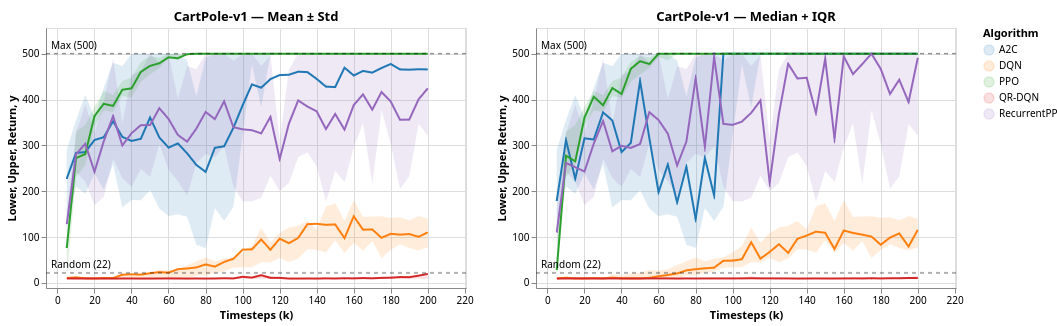
\includegraphics[width=\linewidth]{4_exp1_classic_control/assets/learning_curves_cartpole-v2.png}
  \caption[EXP1: Learning curves, CartPole-v1]{Learning curves for CartPole-v1.PPO and A2C converge to the maximum return of 500 within 100K steps while DQN and QR-DQN fail to learn within the 200K-step budget, with QR-DQN barely moving.}
  \label{fig:lc-cartpole}
\end{figure}

PPO achieves a perfect normalised IQM of $1.000$ $[1.000,\;1.000]$ with
zero variance: all 15 seeds reach the maximum return of 500. A2C also
reaches IQM $1.000$ but with a wider confidence interval
$[0.926,\;1.000]$, indicating that a few seeds converge more slowly.

The surprise was the DQN family. DQN achieves IQM $0.175$ and QR-DQN
scores $-0.022$, which is \emph{below the random baseline}. CartPole is the
environment on which DQN was originally demonstrated
\citep{mnih2015human}, so this failure was unexpected. The explanation
is that with SB3's default hyperparameters,
the replay buffer warm-up phase and $\varepsilon$-greedy exploration
schedule consume a large fraction of the 200K-step budget, leaving
insufficient samples for the value network to converge. QR-DQN is worse
because its distributional head has more parameters to fit with the same
data. 

This highlights how default configurations can lead to suboptimal performance for off-policy methods under limited training budgets, and suggests that while longer training would likely allow convergence comparable to A2C and PPO, it would come at a significantly higher computational cost. This is left as future work (see Chapter~\ref{chap:evaluation}).

\subsection{Acrobot-v1}
\label{sec:acrobot}

Acrobot requires swinging a two-link pendulum above a bar. Returns are negative (closer to zero is better), with the truncation limit at $-500$. I expected this to be a somewhat more difficult task than the previous one for all algorithms. Figure~\ref{fig:lc-acrobot} shows the learning curves.

\begin{figure}[htbp!]
  \centering
  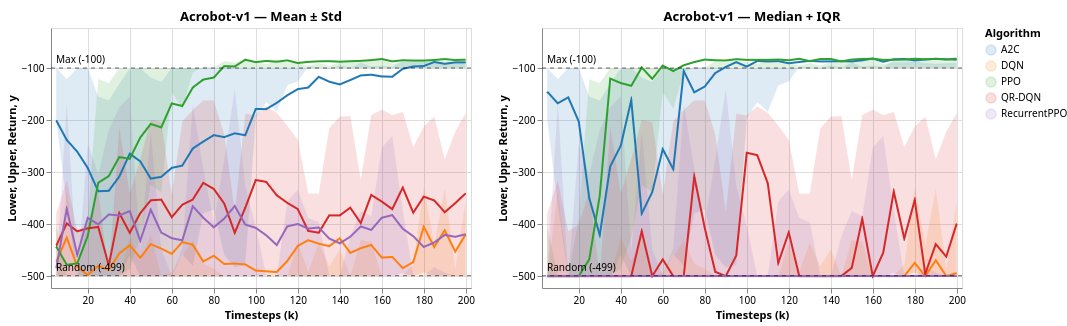
\includegraphics[width=\linewidth]{4_exp1_classic_control/assets/learning_curves_acrobot-v2(correct).png}
  \caption[EXP1: Learning curves, Acrobot-v1]{Learning curves for Acrobot-v1. A2C and PPO both converge near the optimal return ($\approx -85$). RPPO and DQN both fail entirely, remaining near the episode truncation limit of $-500$ throughout training.}
  \label{fig:lc-acrobot}
\end{figure}

PPO and A2C both achieve normalised IQM above 1.0 (PPO: $1.039$, A2C: $1.040$), meaning they consistently beat the reference maximum return. The real unpleasantness was RPPO: it catastrophically fails with IQM $-0.001$, and 12 of its 15 seeds remain stuck at the random-policy floor ($-500$). DQN fares no better—its median stays pinned at $-500$ for the entire training run, with almost no seeds escaping the floor. Unlike RPPO, whose failure stems from unnecessary recurrent capacity complicating the optimisation landscape, DQN's collapse likely reflects its sample-inefficiency on a task where sparse rewards require many steps of credit assignment before any useful gradient signal emerges. This is a fully-observed six-dimensional MDP—the LSTM has nothing useful to remember from the past. Instead, the additional recurrent parameters create an optimisation landscape that gradient descent cannot navigate effectively within 200K steps. More capacity does not mean better performance here. On the contrary, it means strictly worse.

The RPPO collapse on Acrobot is noted as a failure case and discussed further in the limitations section.
\subsection{LunarLander-v3}
\label{sec:lunarlander}

LunarLander is the stress test: an eight-dimensional observation,
four discrete actions, and a 500K-step budget. I expected this to
separate the strong algorithms from the weak ones.
Figure~\ref{fig:lc-lunarlander} confirms this expectation, but with
an unexpected twist.

\begin{figure}[htbp!]
  \centering
  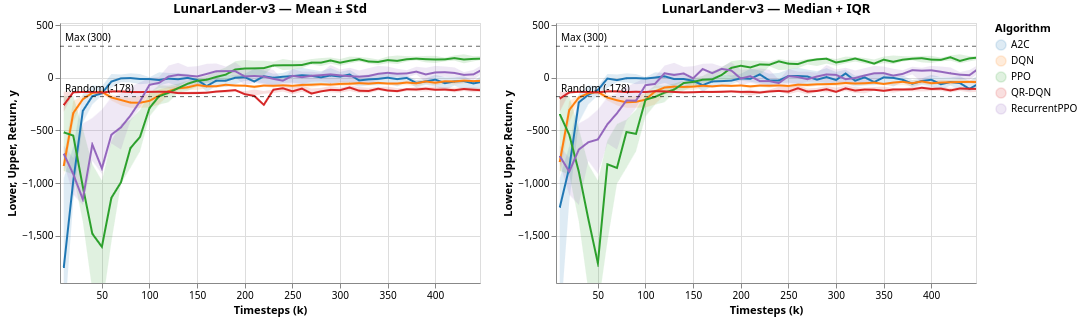
\includegraphics[width=\linewidth]{4_exp1_classic_control/assets/learning_curves_lunarlander-v3.2.png}
  \caption[EXP1: Learning curves, LunarLander-v3]{Learning curves for LunarLander-v3. PPO achieves the highest
           median return ($\approx 230$). A2C learns initially but exhibits
           high variance and eventual performance collapse.}
  \label{fig:lc-lunarlander}
\end{figure}

PPO leads with IQM $0.768$ $[0.714,\;0.814]$---strong but not
dominant. The surprise is A2C's collapse: despite matching PPO on the
other two environments, A2C achieves only IQM $0.303$ here, with an
IQR of $120.9$ raw-reward units. Some seeds learn well; others fail. This bimodal behavior suggests that A2C's single-step updates are too noisy for the longer LunarLander horizon, and the outcome is highly sensitive to the initial random trajectory.

Interestingly, RPPO ($0.444$) outperforms A2C ($0.303$) and DQN
($0.309$) on LunarLander. The LSTM may exploit temporal correlations
in the lander's descent trajectory---the one environment in our suite
where sequential memory plausibly helps.

\subsection{Combined Learning Curves}
\label{sec:combined-lc}

Figure~\ref{fig:lc-combined} overlays all three environments on a
normalised $y$-axis, making the overall pattern clear: PPO and A2C are
the only algorithms that consistently rise above the random baseline
across all tasks.

\begin{figure}[htbp!]
  \centering
  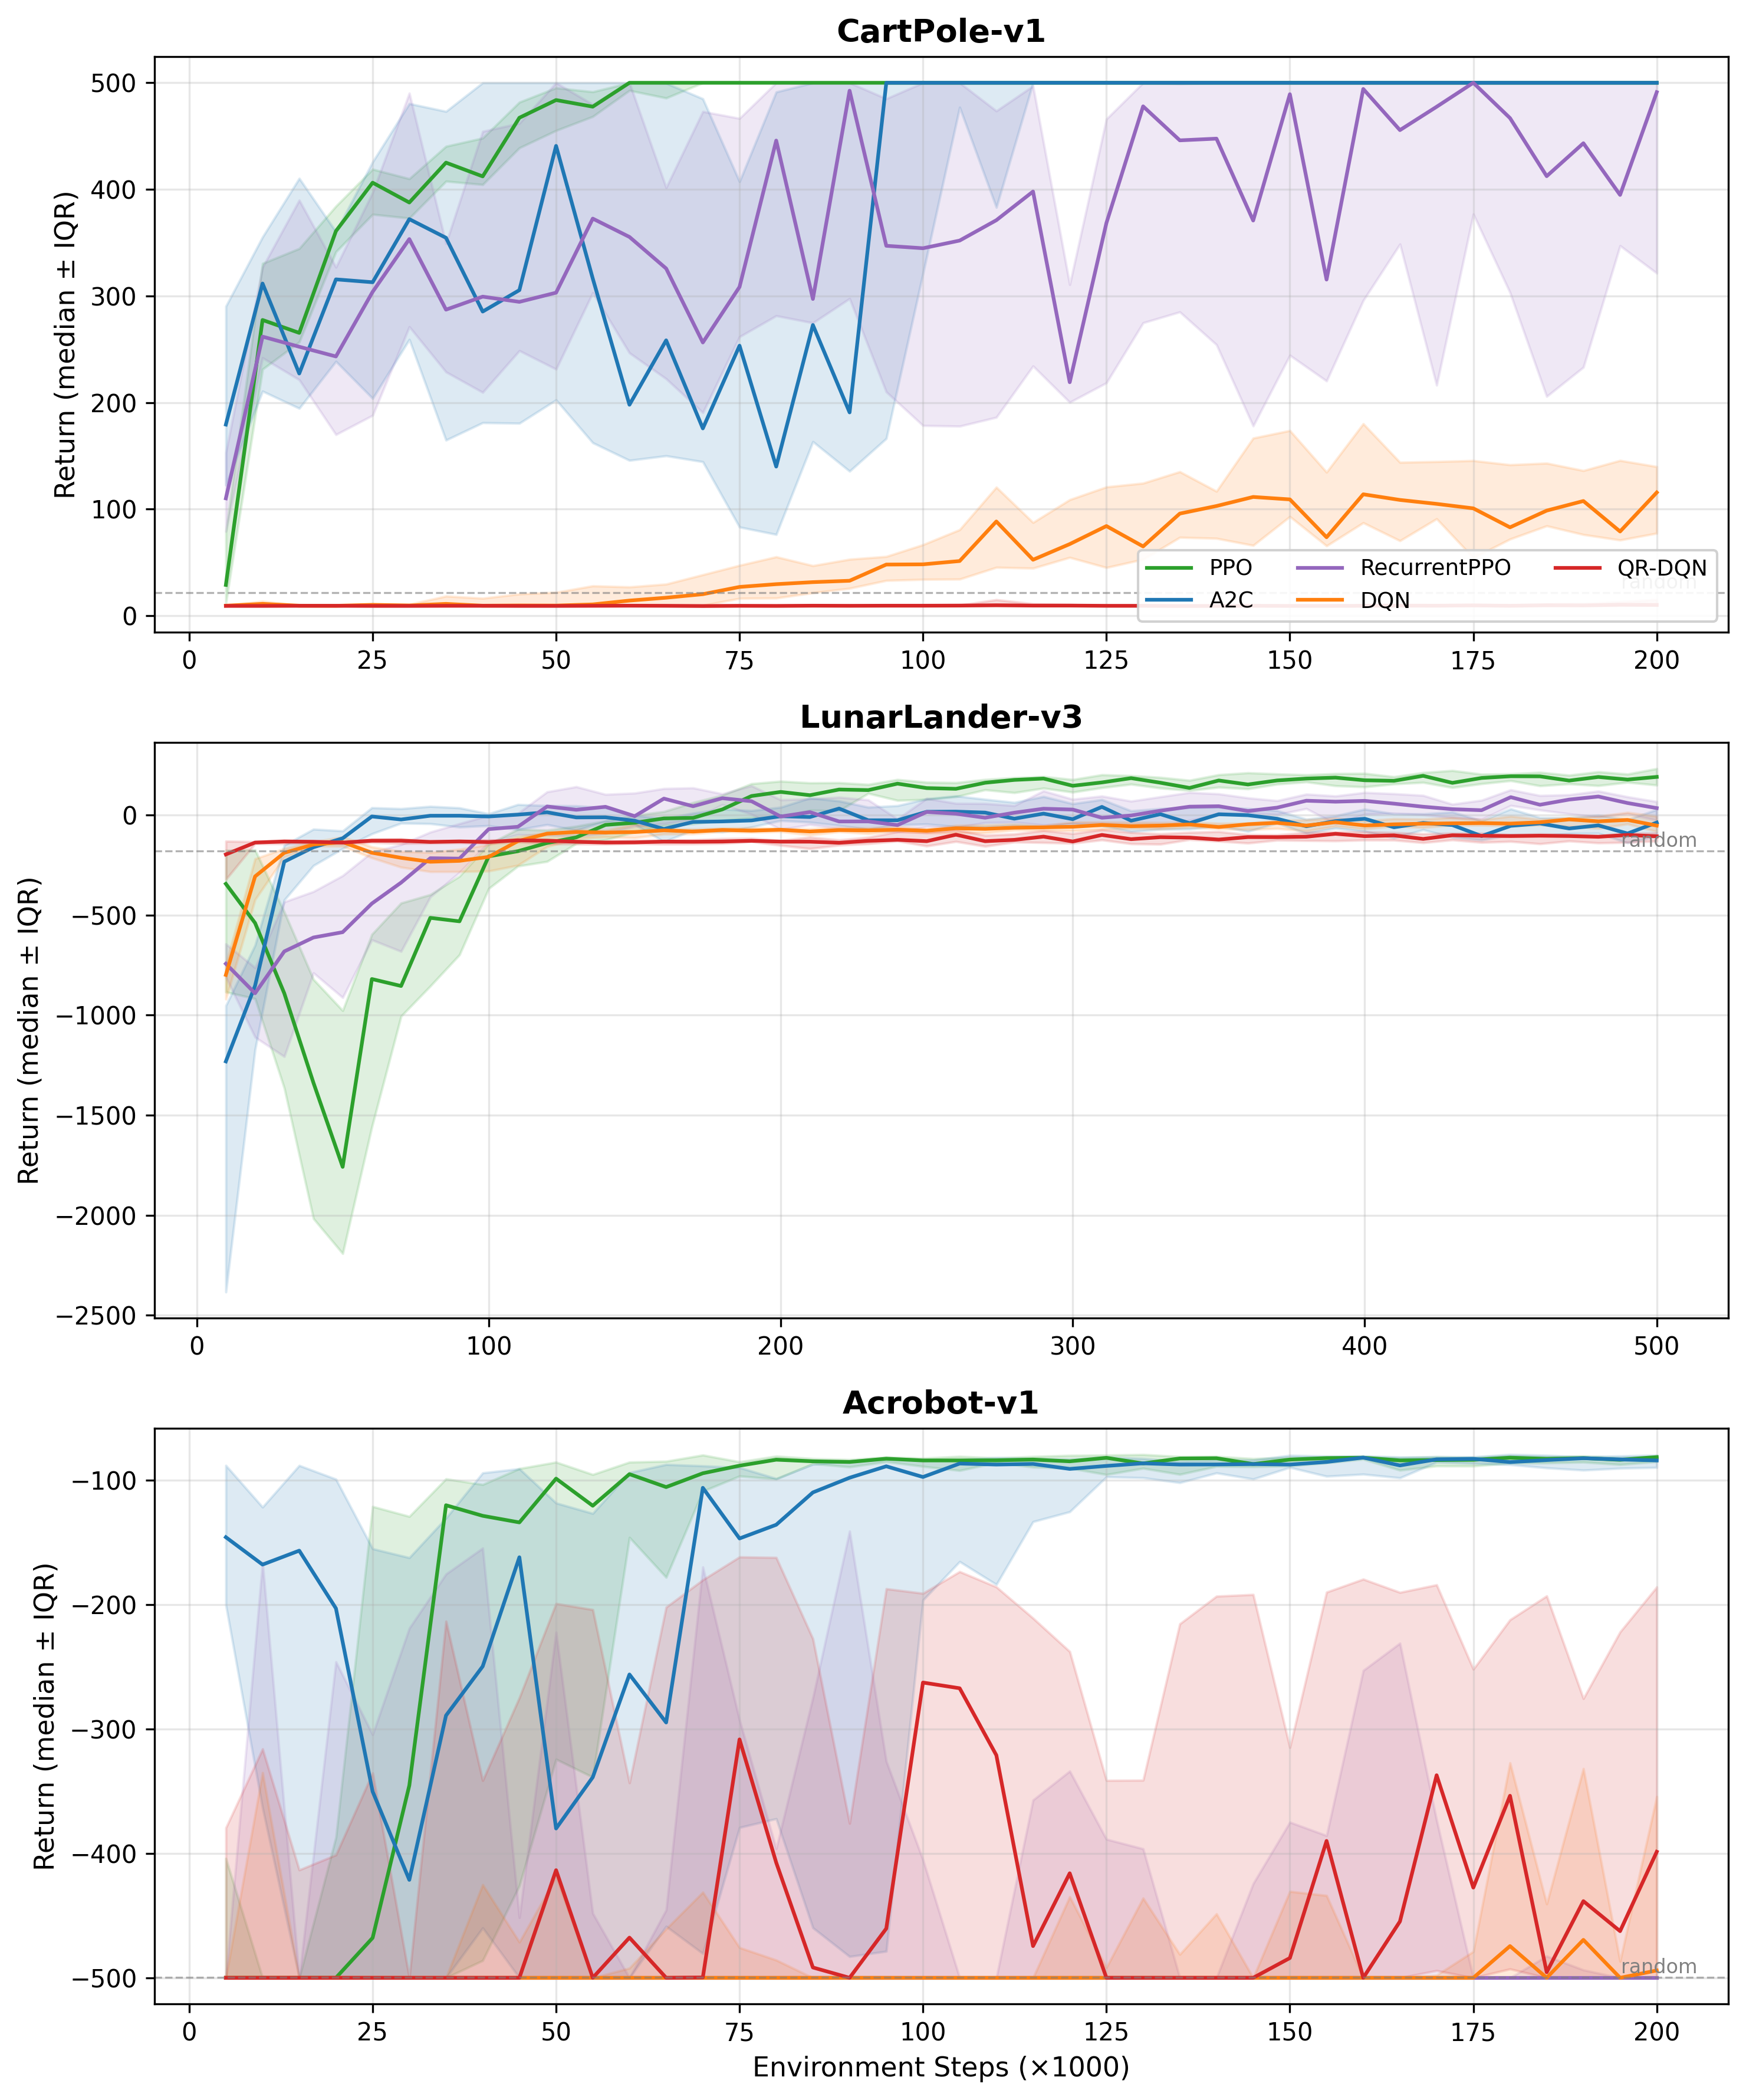
\includegraphics[width=\linewidth]{4_exp1_classic_control/assets/combined_learning_curves.png}
  \caption[EXP1: Combined learning curves]{Combined normalized learning curves across all three
           environments. PPO and A2C are the only algorithms that
           consistently rise above the random baseline across all tasks.
}
  \label{fig:lc-combined}
\end{figure}

\subsection{Score Distributions and Per-Seed Analysis}
\label{sec:score-dist}

% Figures~\ref{fig:score-dist},~\ref{fig:heatmap},and~\ref{fig:boxswarm} 
Figures,~\ref{fig:boxswarm}, and~\ref{fig:heatmap} provide complementary views of the per-seed results. The score distribution (Figure~\ref{fig:boxswarm}) confirms PPO's concentration near 1.0 and reveals A2C's bimodality and highlights anomalous seeds (marked with red crosses) that fall below the random baseline.
The heatmap (Figure~\ref{fig:heatmap}) exposes RPPO's
environment-specific failure on Acrobot as a wall of red.


% \begin{figure}[htbp!]
%   \centering
%   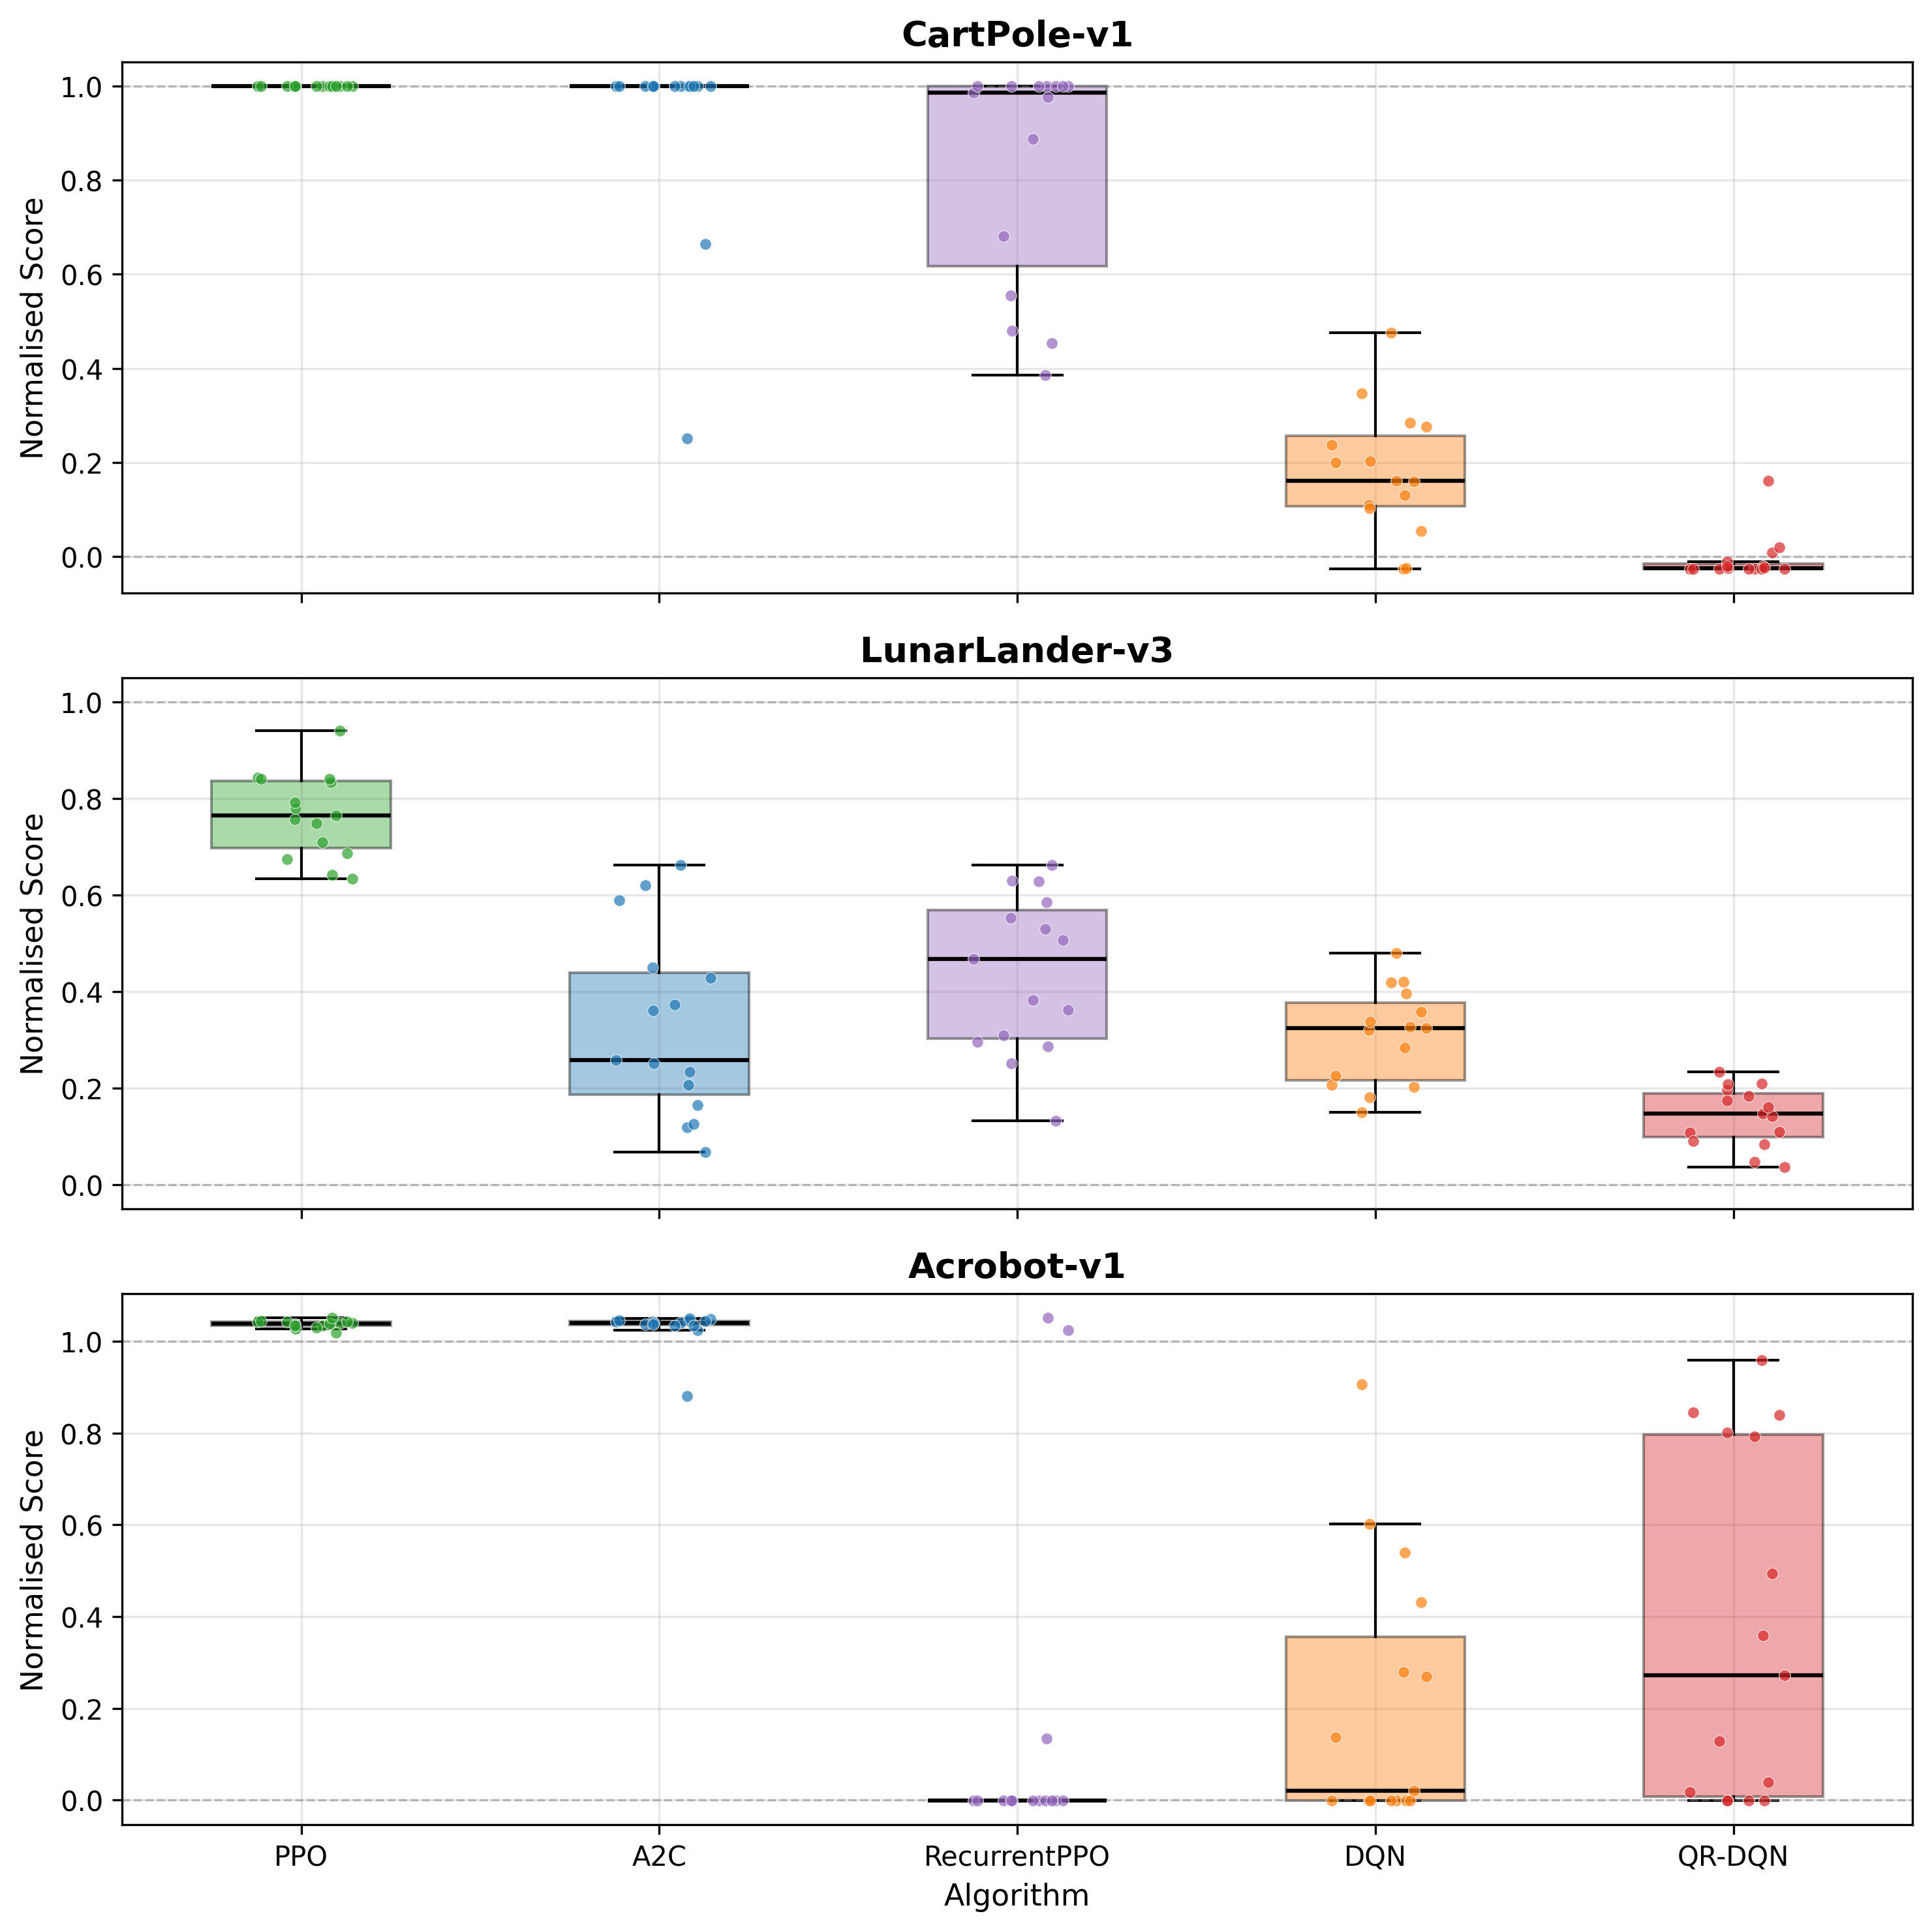
\includegraphics[width=\linewidth]{4_exp1_classic_control/assets/score_distribution.png}
%   \caption{Distribution of normalised scores per environment. PPO is
%            concentrated near 1.0; A2C is bimodal (strong on CartPole and
%            Acrobot, weak on LunarLander); DQN and QR-DQN are concentrated
%            near zero.
% }
%   \label{fig:score-dist}
% \end{figure}

\begin{figure}[htbp!]
  \centering
  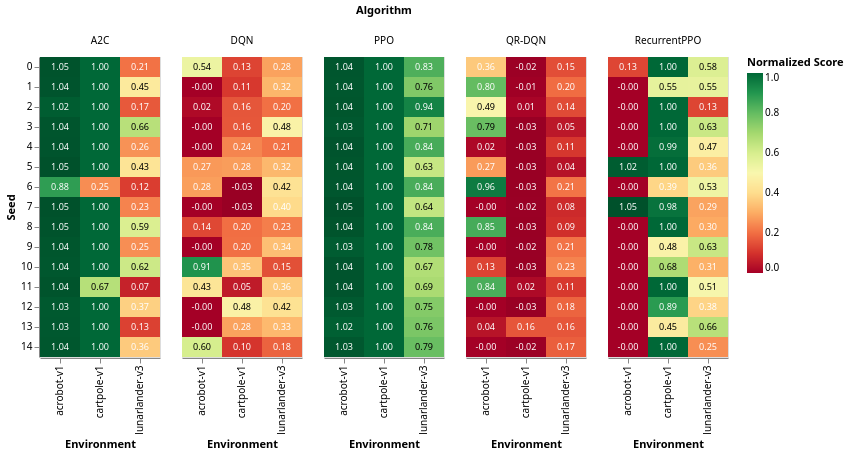
\includegraphics[width=\linewidth]{4_exp1_classic_control/assets/per_seed_heatmap2.png}
  \caption[EXP1: Per-seed score heatmap]{Heatmap of normalised final scores by seed and environment.
           Each row is one of 15 seeds; columns are environments.
           PPO achieves uniformly high scores. RPPO shows a clear
           environment-dependent failure mode on Acrobot.
}
  \label{fig:heatmap}
\end{figure}

\begin{figure}[htbp!]
  \centering
  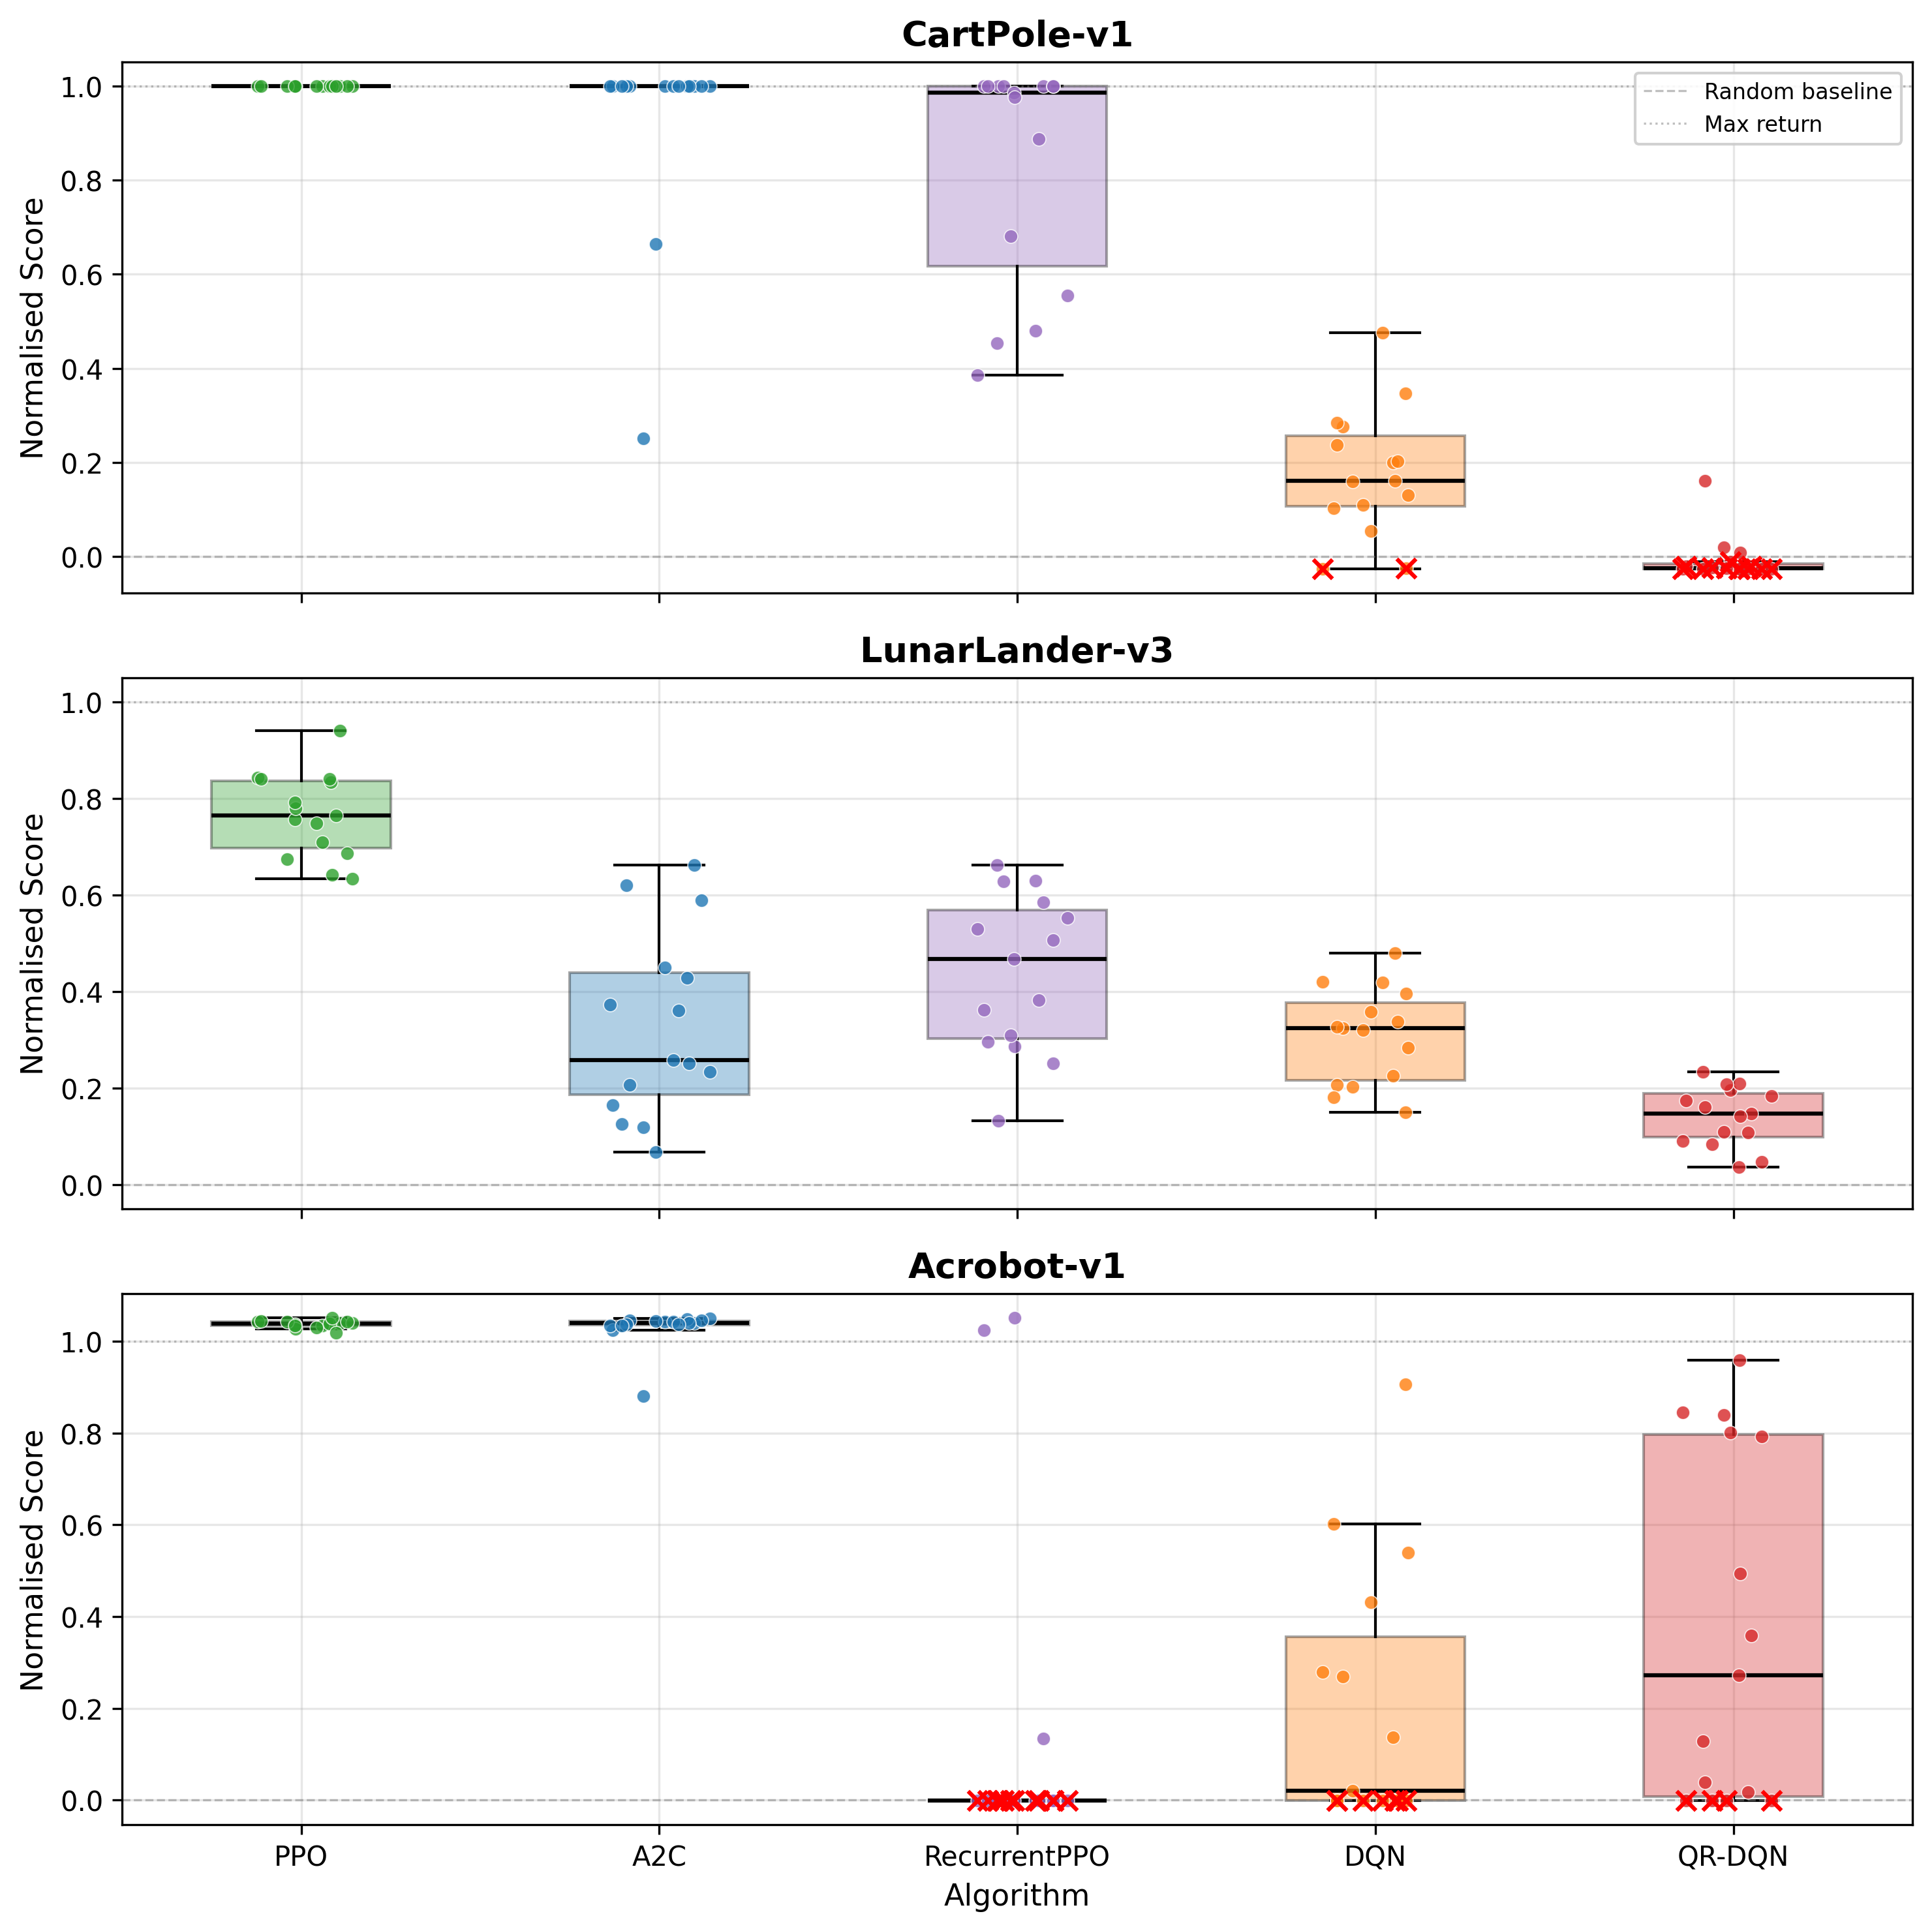
\includegraphics[width=\linewidth]{4_exp1_classic_control/assets/per_seed_boxswarm.png}
  \caption[EXP1: Per-seed score spread]{Box-and-swarm plot of per-seed normalised scores. Individual
           seeds are shown as dots; boxes indicate the IQR. A2C exhibits
           the widest spread on LunarLander; PPO has near-zero variance
           on CartPole and Acrobot. Red crosses mark seeds below the
           random baseline.
}
  \label{fig:boxswarm}
\end{figure}

Table~\ref{tab:per-env-iqm} summarises the per-environment normalised
IQM with 95\% bootstrap confidence intervals.

\begin{table}[htbp!]
\centering
\caption[EXP1: Per-environment IQM]{Per-environment normalised IQM with 95\% bootstrap CIs.}
\label{tab:per-env-iqm}
\begin{tabular}{lccc}
\toprule
\textbf{Algorithm} & \textbf{CartPole-v1} & \textbf{LunarLander-v3}
                   & \textbf{Acrobot-v1} \\
\midrule
PPO    & $1.000\;[1.000,\;1.000]$ & $0.768\;[0.714,\;0.814]$
       & $1.039\;[1.034,\;1.042]$ \\
A2C    & $1.000\;[0.926,\;1.000]$ & $0.303\;[0.204,\;0.438]$
       & $1.040\;[1.035,\;1.044]$ \\
RPPO   & $0.898\;[0.704,\;0.997]$ & $0.444\;[0.343,\;0.548]$
       & $-0.001\;[-0.001,\;0.241]$ \\
DQN    & $0.175\;[0.104,\;0.242]$ & $0.309\;[0.249,\;0.368]$
       & $0.126\;[0.003,\;0.328]$ \\
QR-DQN & $-0.022\;[-0.025,\;-0.007]$ & $0.146\;[0.107,\;0.181]$
       & $0.322\;[0.077,\;0.622]$ \\
\bottomrule
\end{tabular}
\end{table}

%% ------------------------------------------------------------------
\section{Cross-Environment Aggregate Results}
\label{sec:cross-env-results}

\subsection{Final Performance}
\label{sec:final-perf}

Table~\ref{tab:cross-env} reports the cross-environment aggregate metrics
at the final training budget. PPO achieves the highest IQM ($0.981$) with
the tightest confidence interval and the smallest optimality gap ($0.078$).

\begin{table}[htbp!]
\centering
\caption[EXP1: Cross-environment aggregate metrics]{Cross-environment aggregate metrics (normalised scores). IQM,
         mean, and median are reported with 95\% bootstrap CIs.}
\label{tab:cross-env}
\begin{tabular}{lcccc}
\toprule
\textbf{Algorithm} & \textbf{IQM} & \textbf{Mean} & \textbf{Median}
                   & \textbf{Opt.\ Gap} \\
\midrule
PPO    & $0.981\;[0.971,\;0.991]$ & $0.934\;[0.912,\;0.953]$
       & $1.000$ & $0.078\;[0.064,\;0.092]$ \\
A2C    & $0.886\;[0.807,\;0.934]$ & $0.762\;[0.713,\;0.805]$
       & $0.928$ & $0.251\;[0.208,\;0.299]$ \\
RPPO   & $0.442\;[0.345,\;0.583]$ & $0.471\;[0.382,\;0.556]$
       & $0.439$ & $0.531\;[0.454,\;0.601]$ \\
DQN    & $0.222\;[0.164,\;0.276]$ & $0.233\;[0.186,\;0.280]$
       & $0.212$ & $0.767\;[0.710,\;0.818]$ \\
QR-DQN & $0.080\;[0.045,\;0.121]$ & $0.168\;[0.115,\;0.225]$
       & $0.142$ & $0.832\;[0.768,\;0.893]$ \\
\bottomrule
\end{tabular}
\end{table}

\begin{figure}[htbp!]
  \centering
  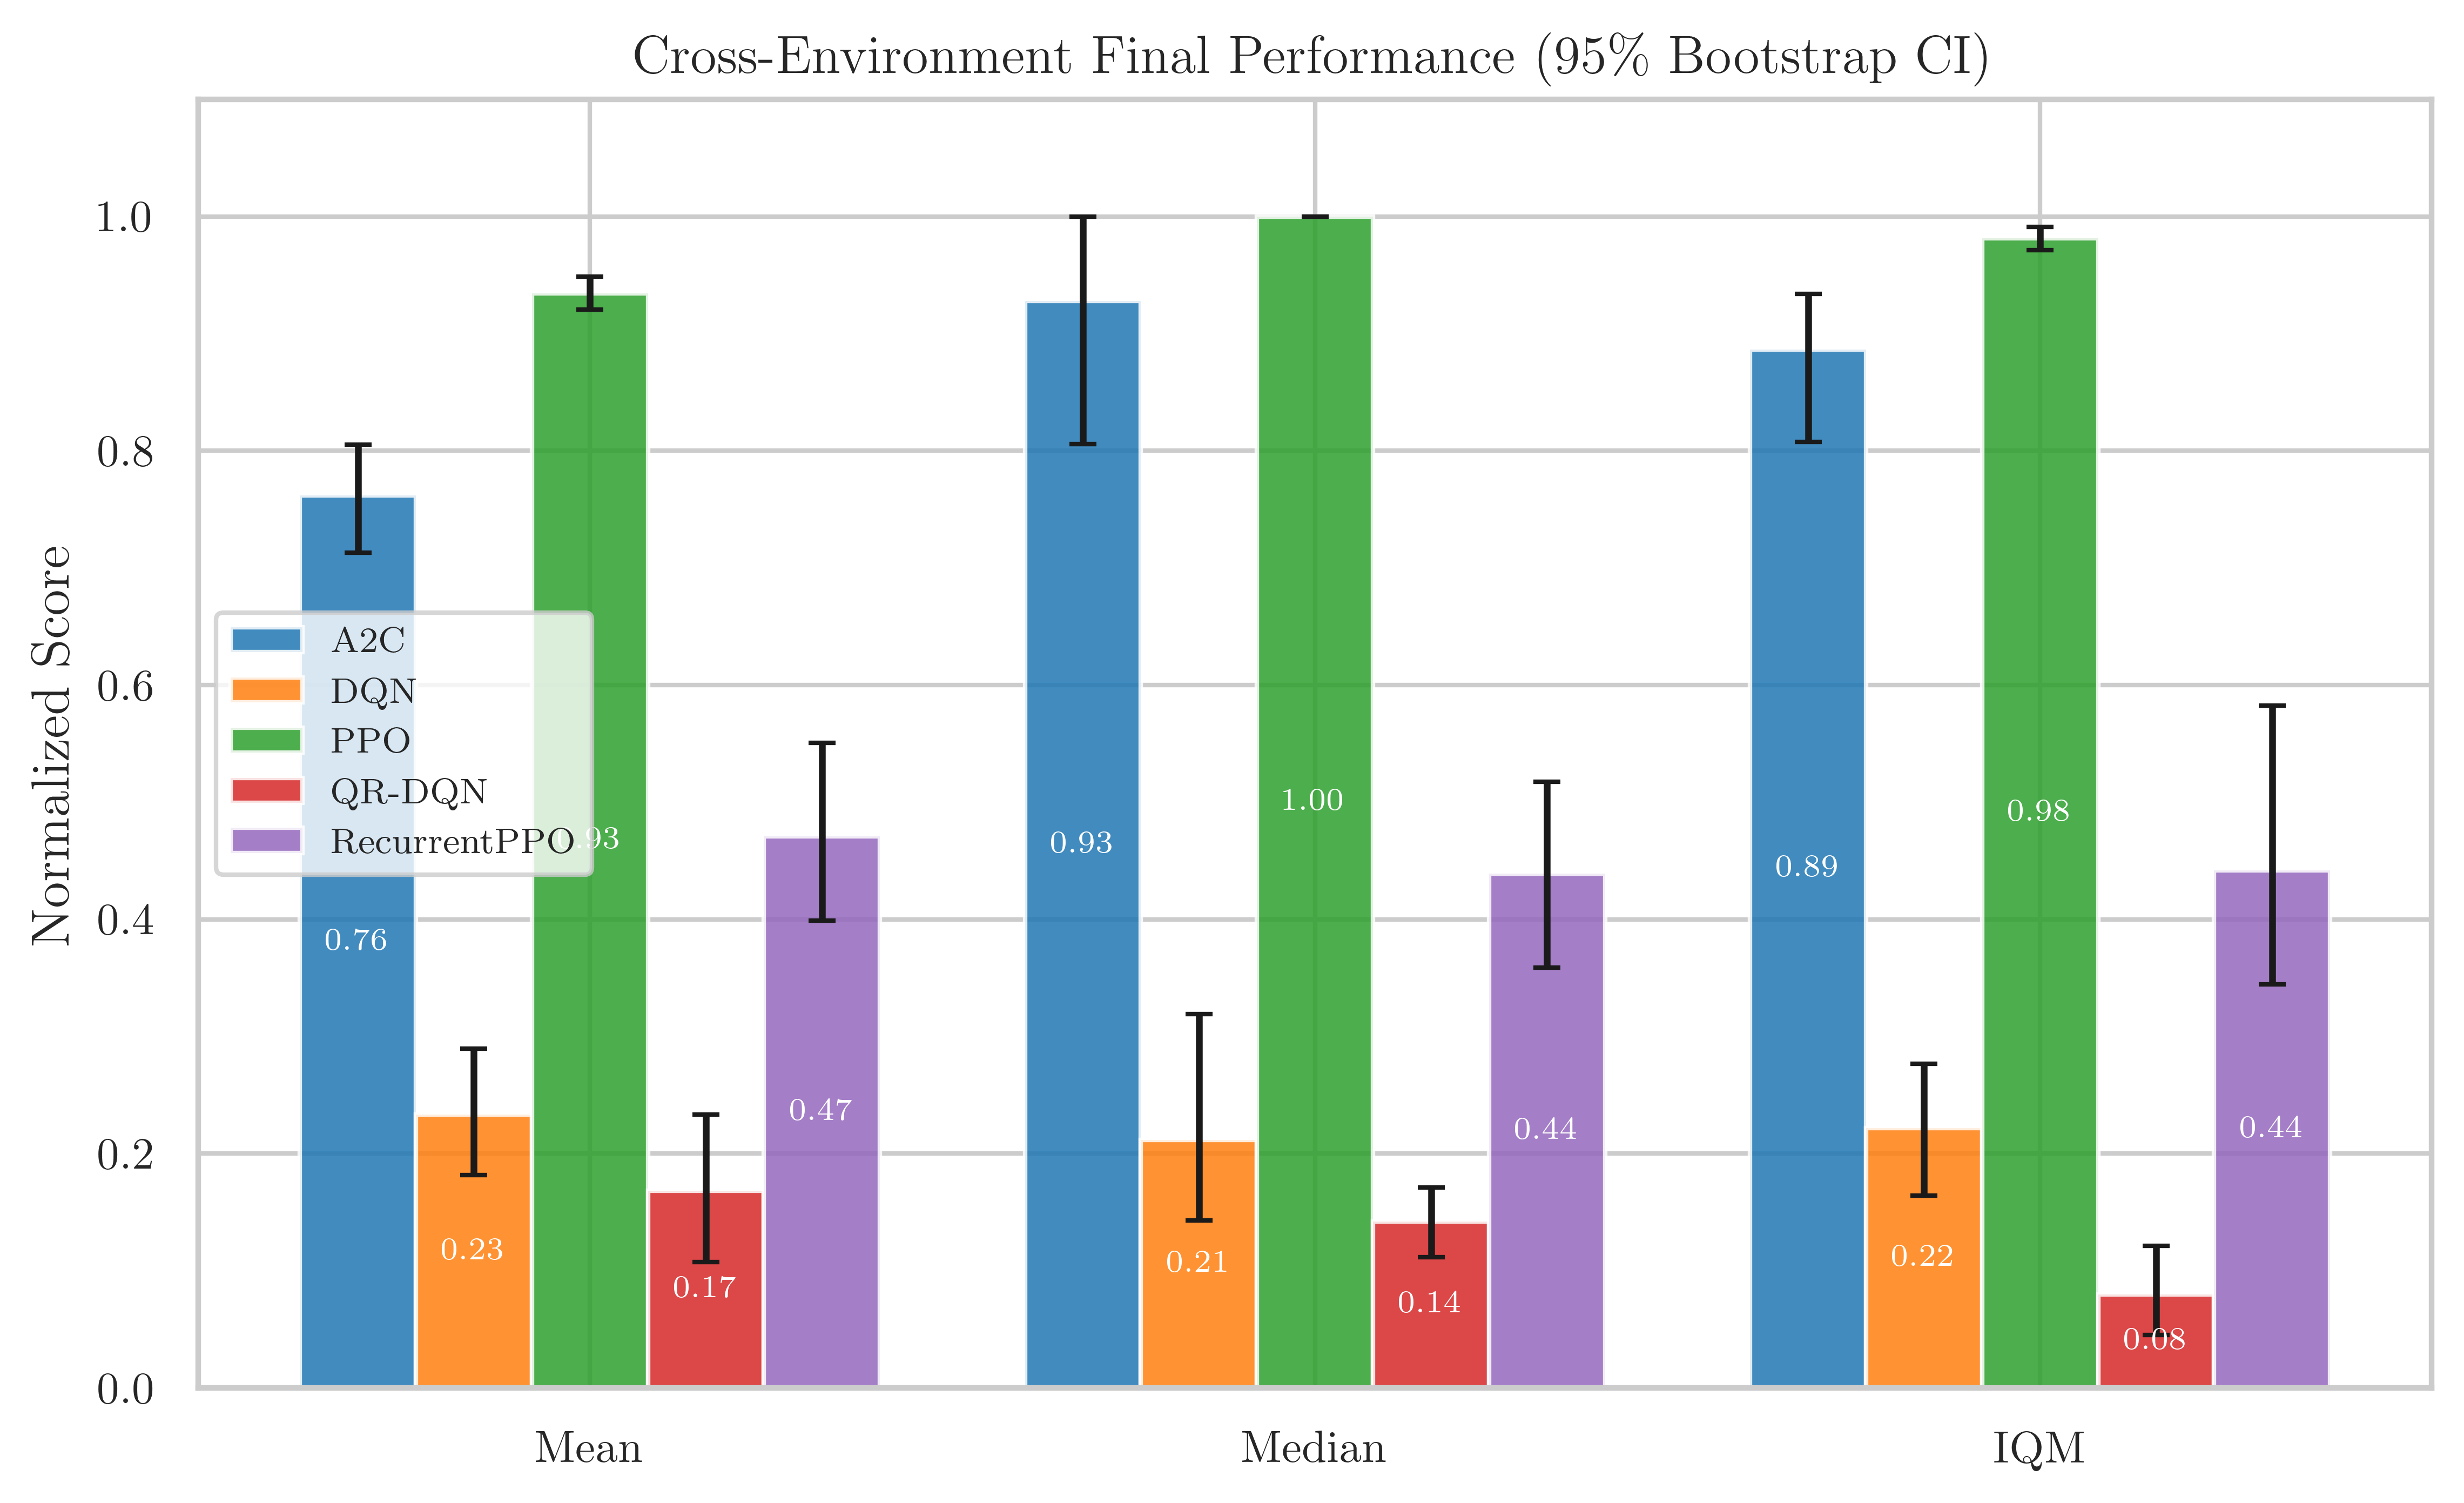
\includegraphics[width=\linewidth]{4_exp1_classic_control/assets/final_performance.png}
  \caption[EXP1: Cross-environment IQM]{Cross-environment IQM, mean, and median with 95\% bootstrap
           confidence intervals.}
  \label{fig:final-perf}
\end{figure}

\subsection{Performance Profile and Optimality Gap}
\label{sec:profile-gap}

The performance profile (Figure~\ref{fig:perf-profile}) shows the fraction of runs exceeding the normalized score $\tau$. PPO maintains $\hat{F}(\tau) > 0.9$ up to $\tau \approx 0.8$, so most runs stay close to the top. In contrast, DQN and QR-DQN fall below 50\% at $\tau = 0.3$, indicating that, in most cases, they do not even reach moderate performance. Overall, PPO is not just better on average but also much more reliable, whereas the DQN variants are inconsistent and often fail under the same setup.

\begin{figure}[htbp!]
  \centering
  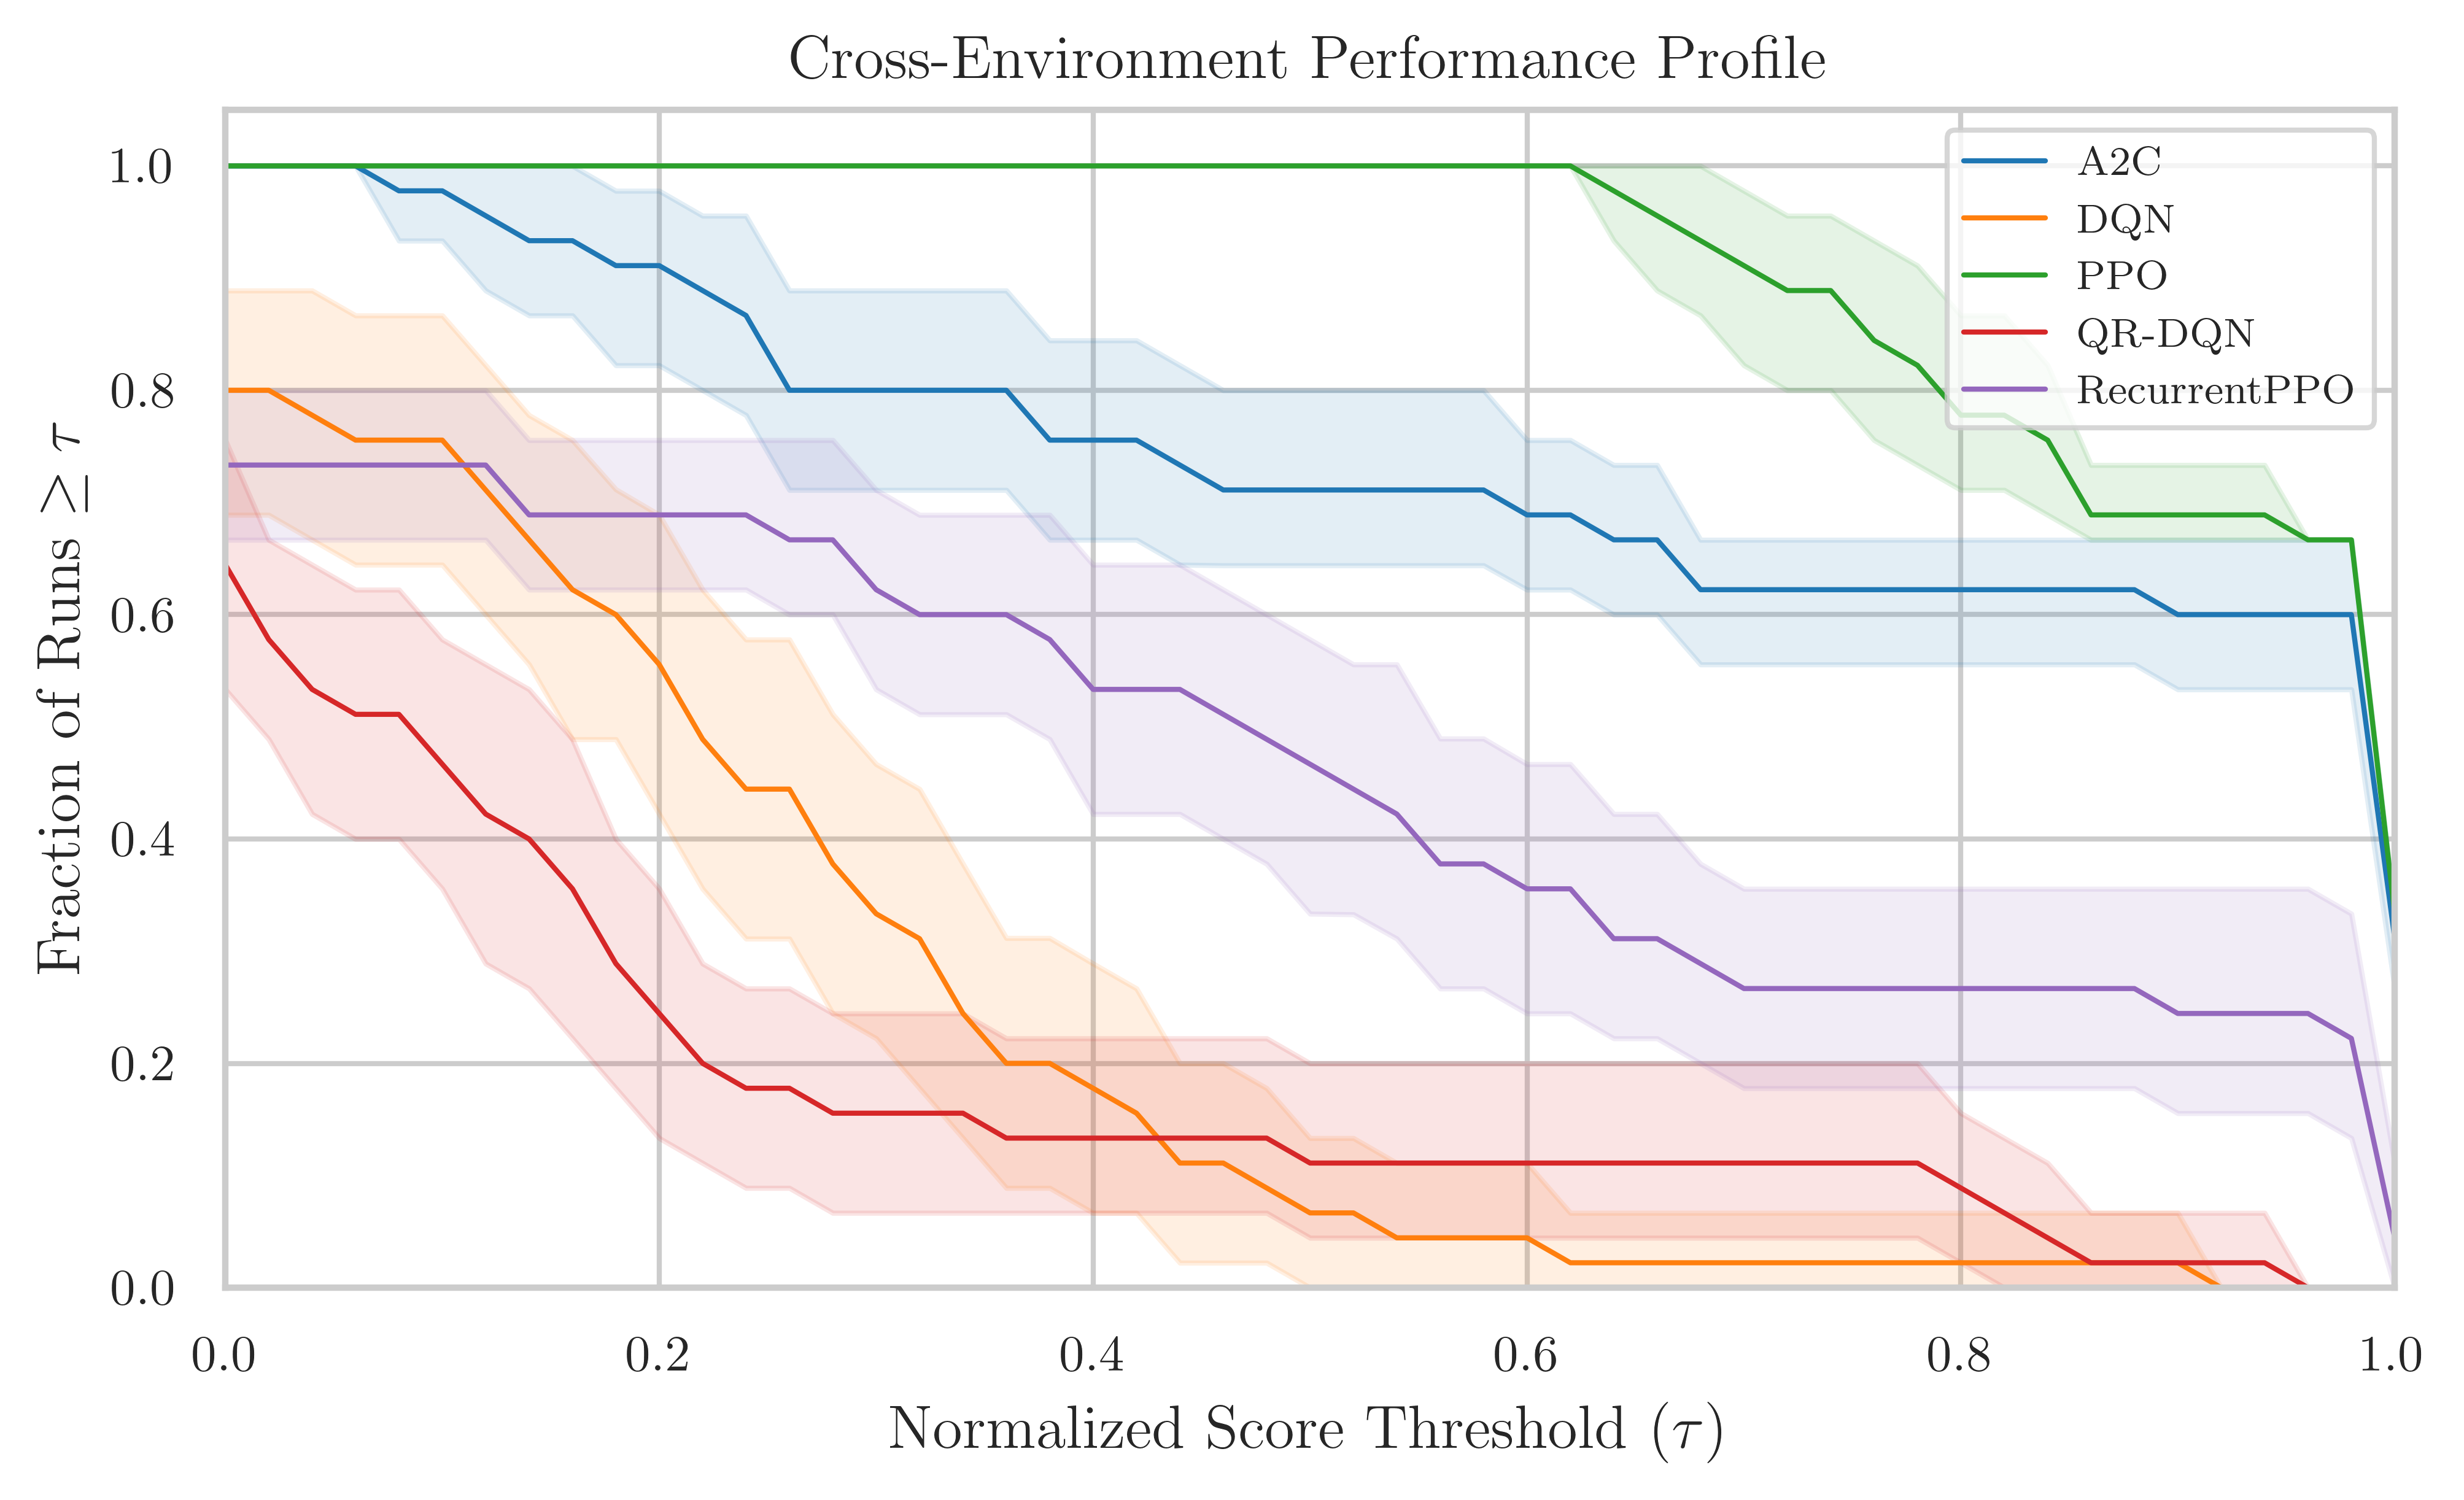
\includegraphics[width=\linewidth]{4_exp1_classic_control/assets/performance_profile.png}
  \caption[EXP1: Performance profiles]{Performance profiles with 95\% bootstrap CIs. Higher curves
           indicate a larger fraction of runs exceeding each score
           threshold $\tau$.}
  \label{fig:perf-profile}
\end{figure}

\begin{figure}[htbp!]
  \centering
  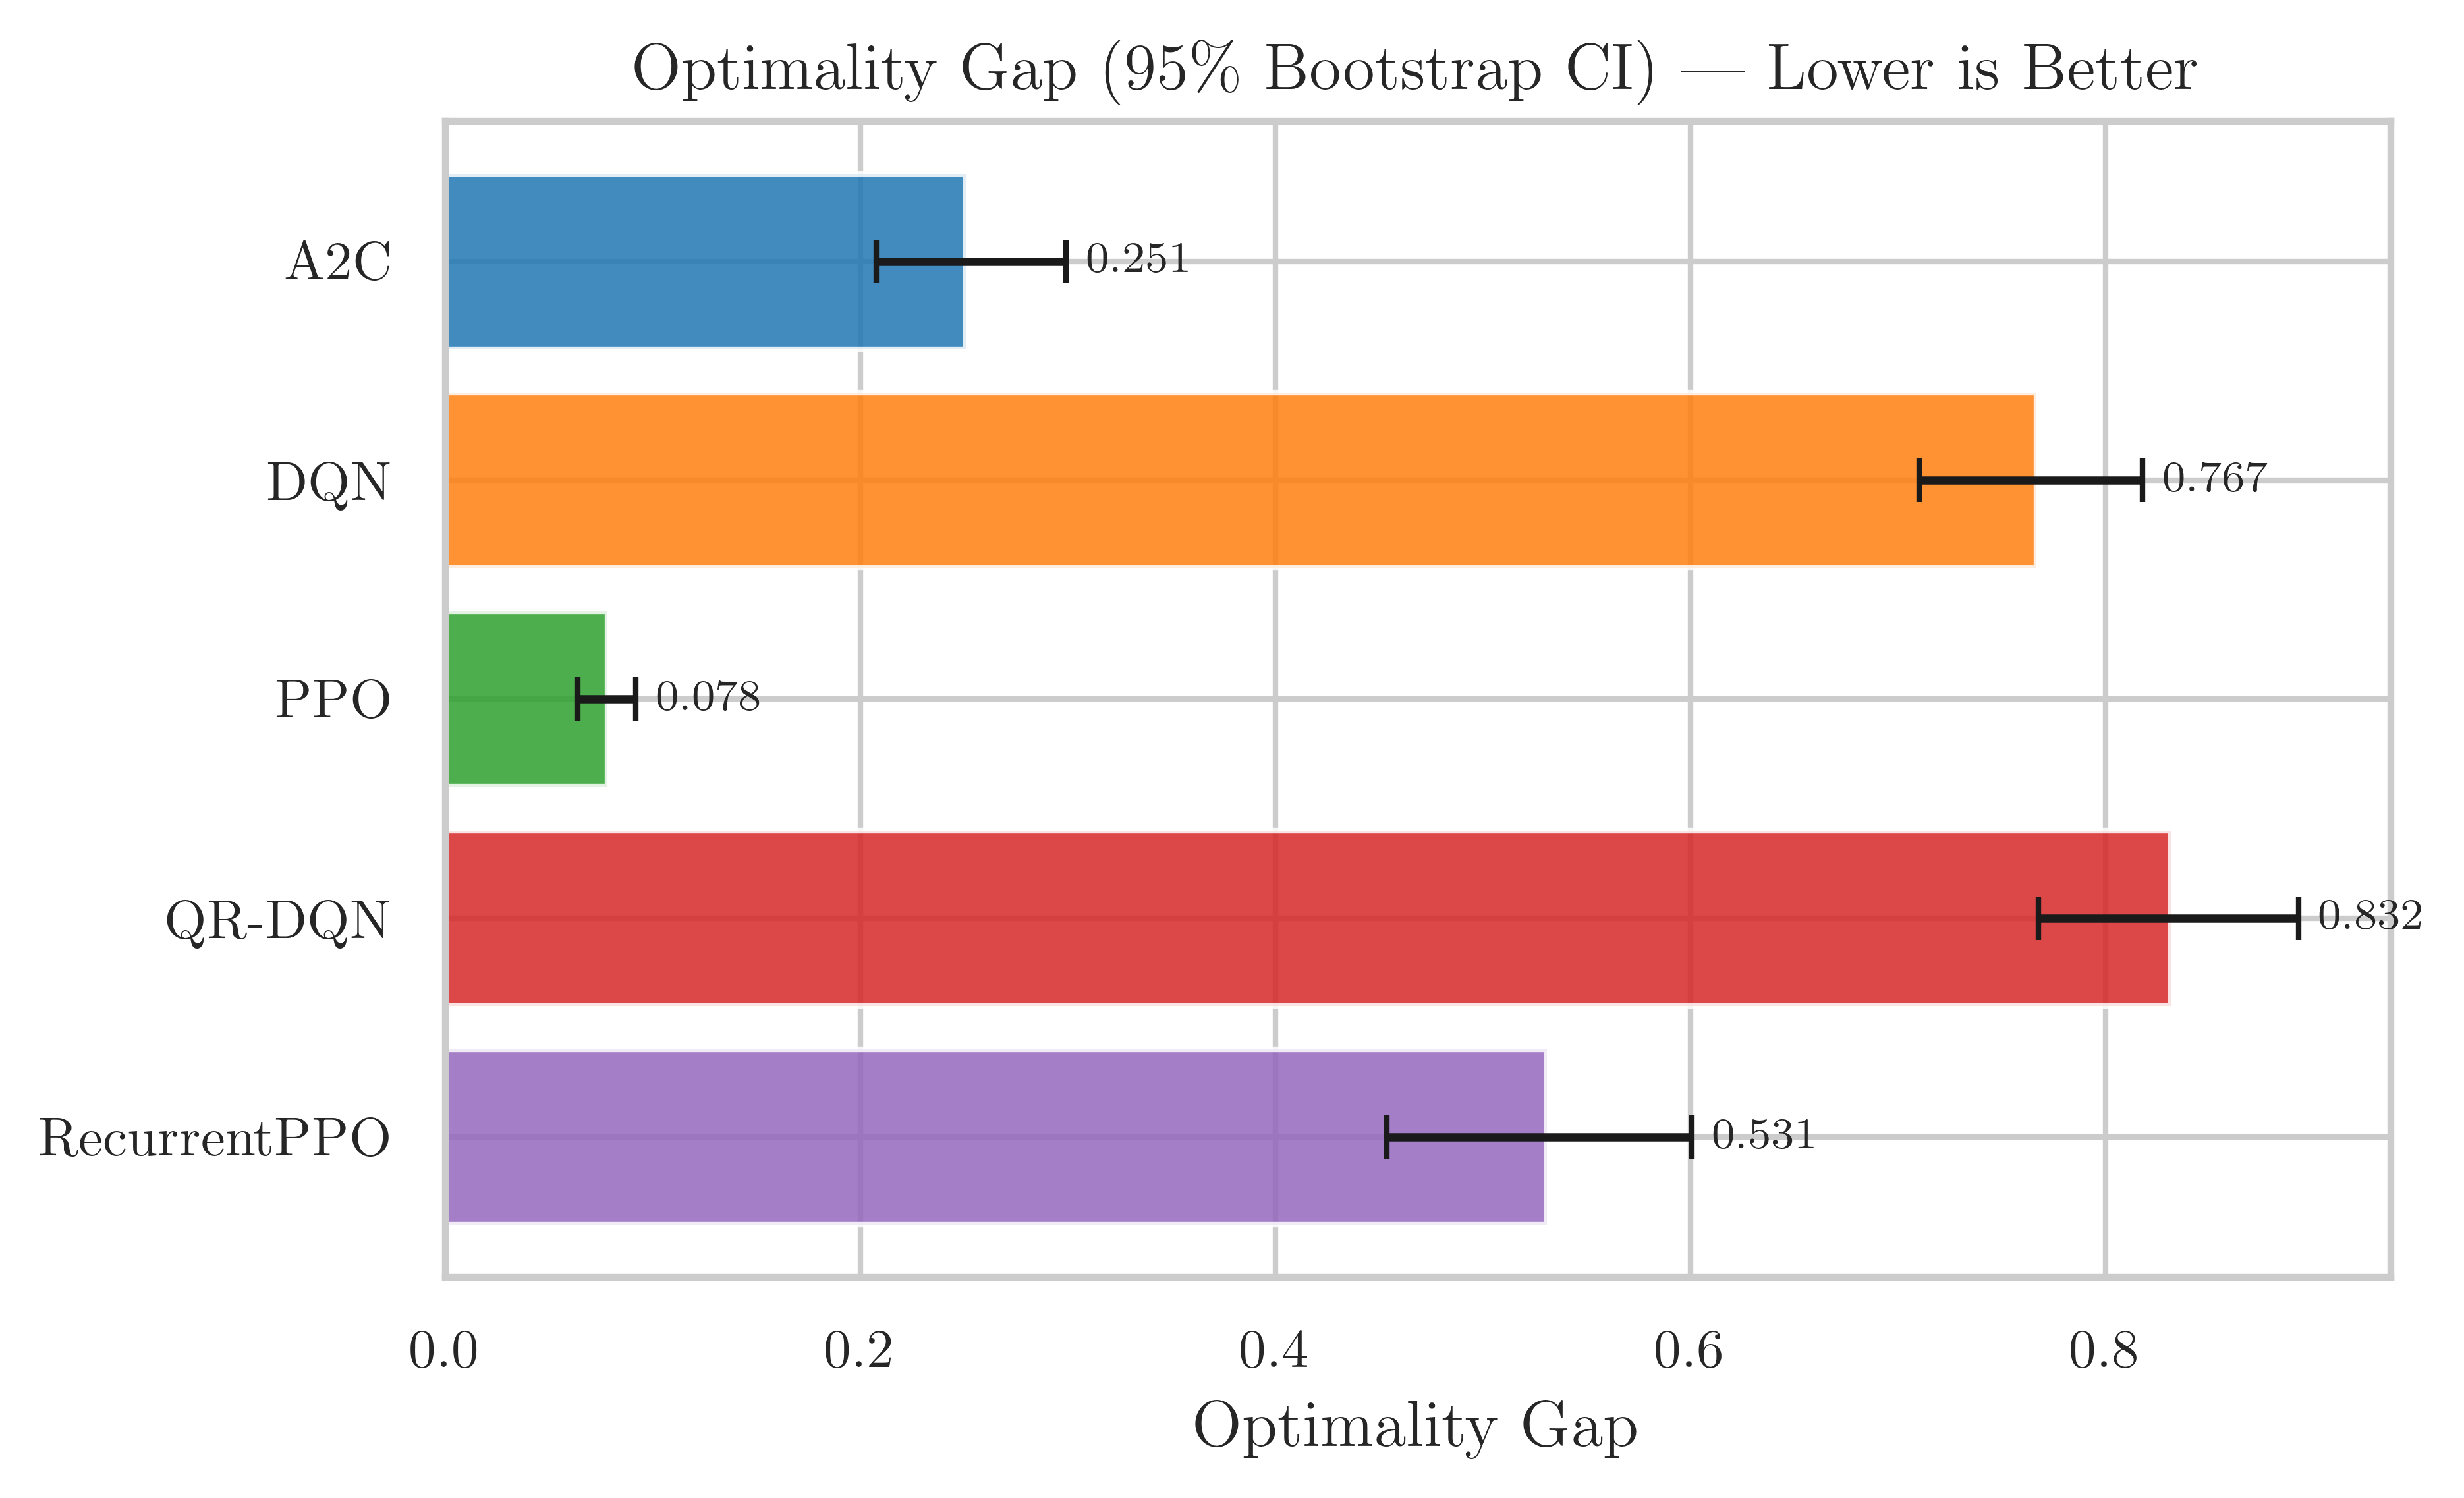
\includegraphics[width=\linewidth]{4_exp1_classic_control/assets/optimality_gap.png}
  \caption[EXP1: Optimality gap]{Optimality gap with 95\% bootstrap CIs. Lower values indicate
           smaller shortfall from the target. PPO ($0.078$) has the
           smallest gap; QR-DQN ($0.832$) has the largest.}
  \label{fig:opt-gap}
\end{figure}

\subsection{Sample Efficiency}
\label{sec:sample-eff}

Figures~\ref{fig:se-cartpole}--\ref{fig:se-acrobot} show sample
efficiency as normalised Area Under the Learning Curve (AUC) over the training budget.

\begin{figure}[htbp!]
  \centering
  \begin{subfigure}[b]{0.5\linewidth}
    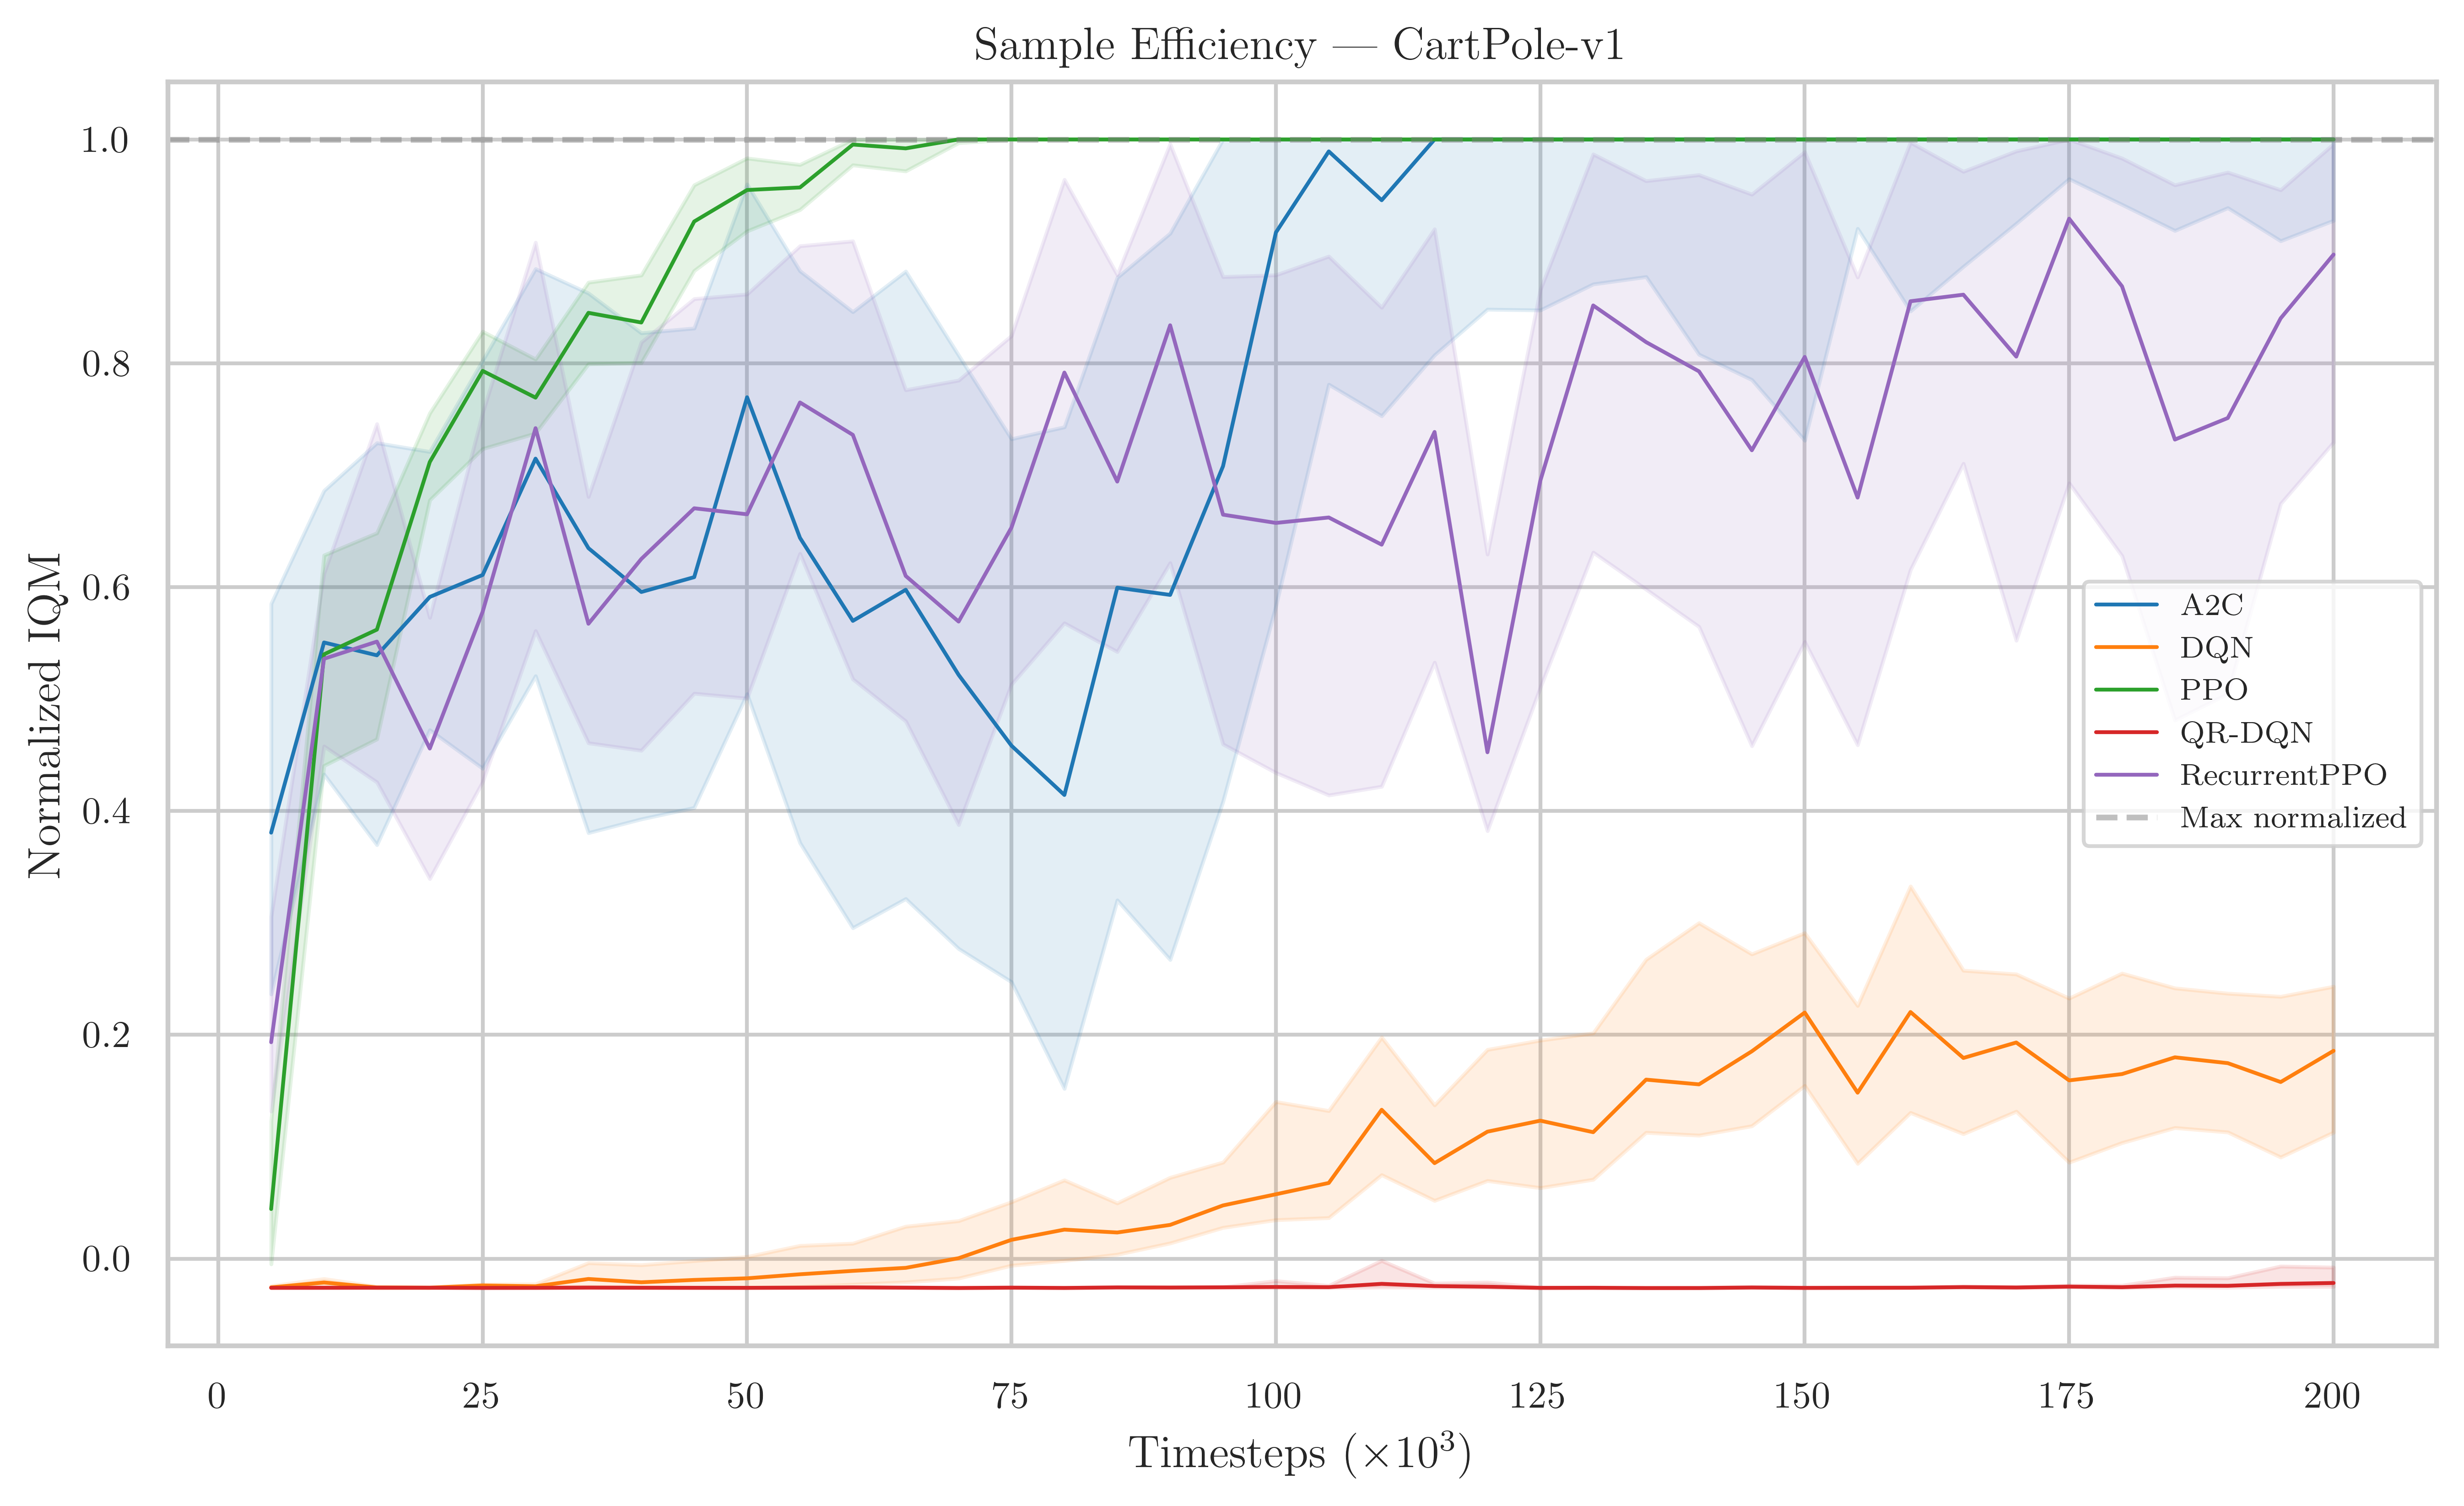
\includegraphics[width=\linewidth]{4_exp1_classic_control/assets/sample_efficiency_cartpole-v1.png}
    \caption{CartPole-v1}
    \label{fig:se-cartpole}
  \end{subfigure}
  \hfill
  \begin{subfigure}[b]{0.5\linewidth}
    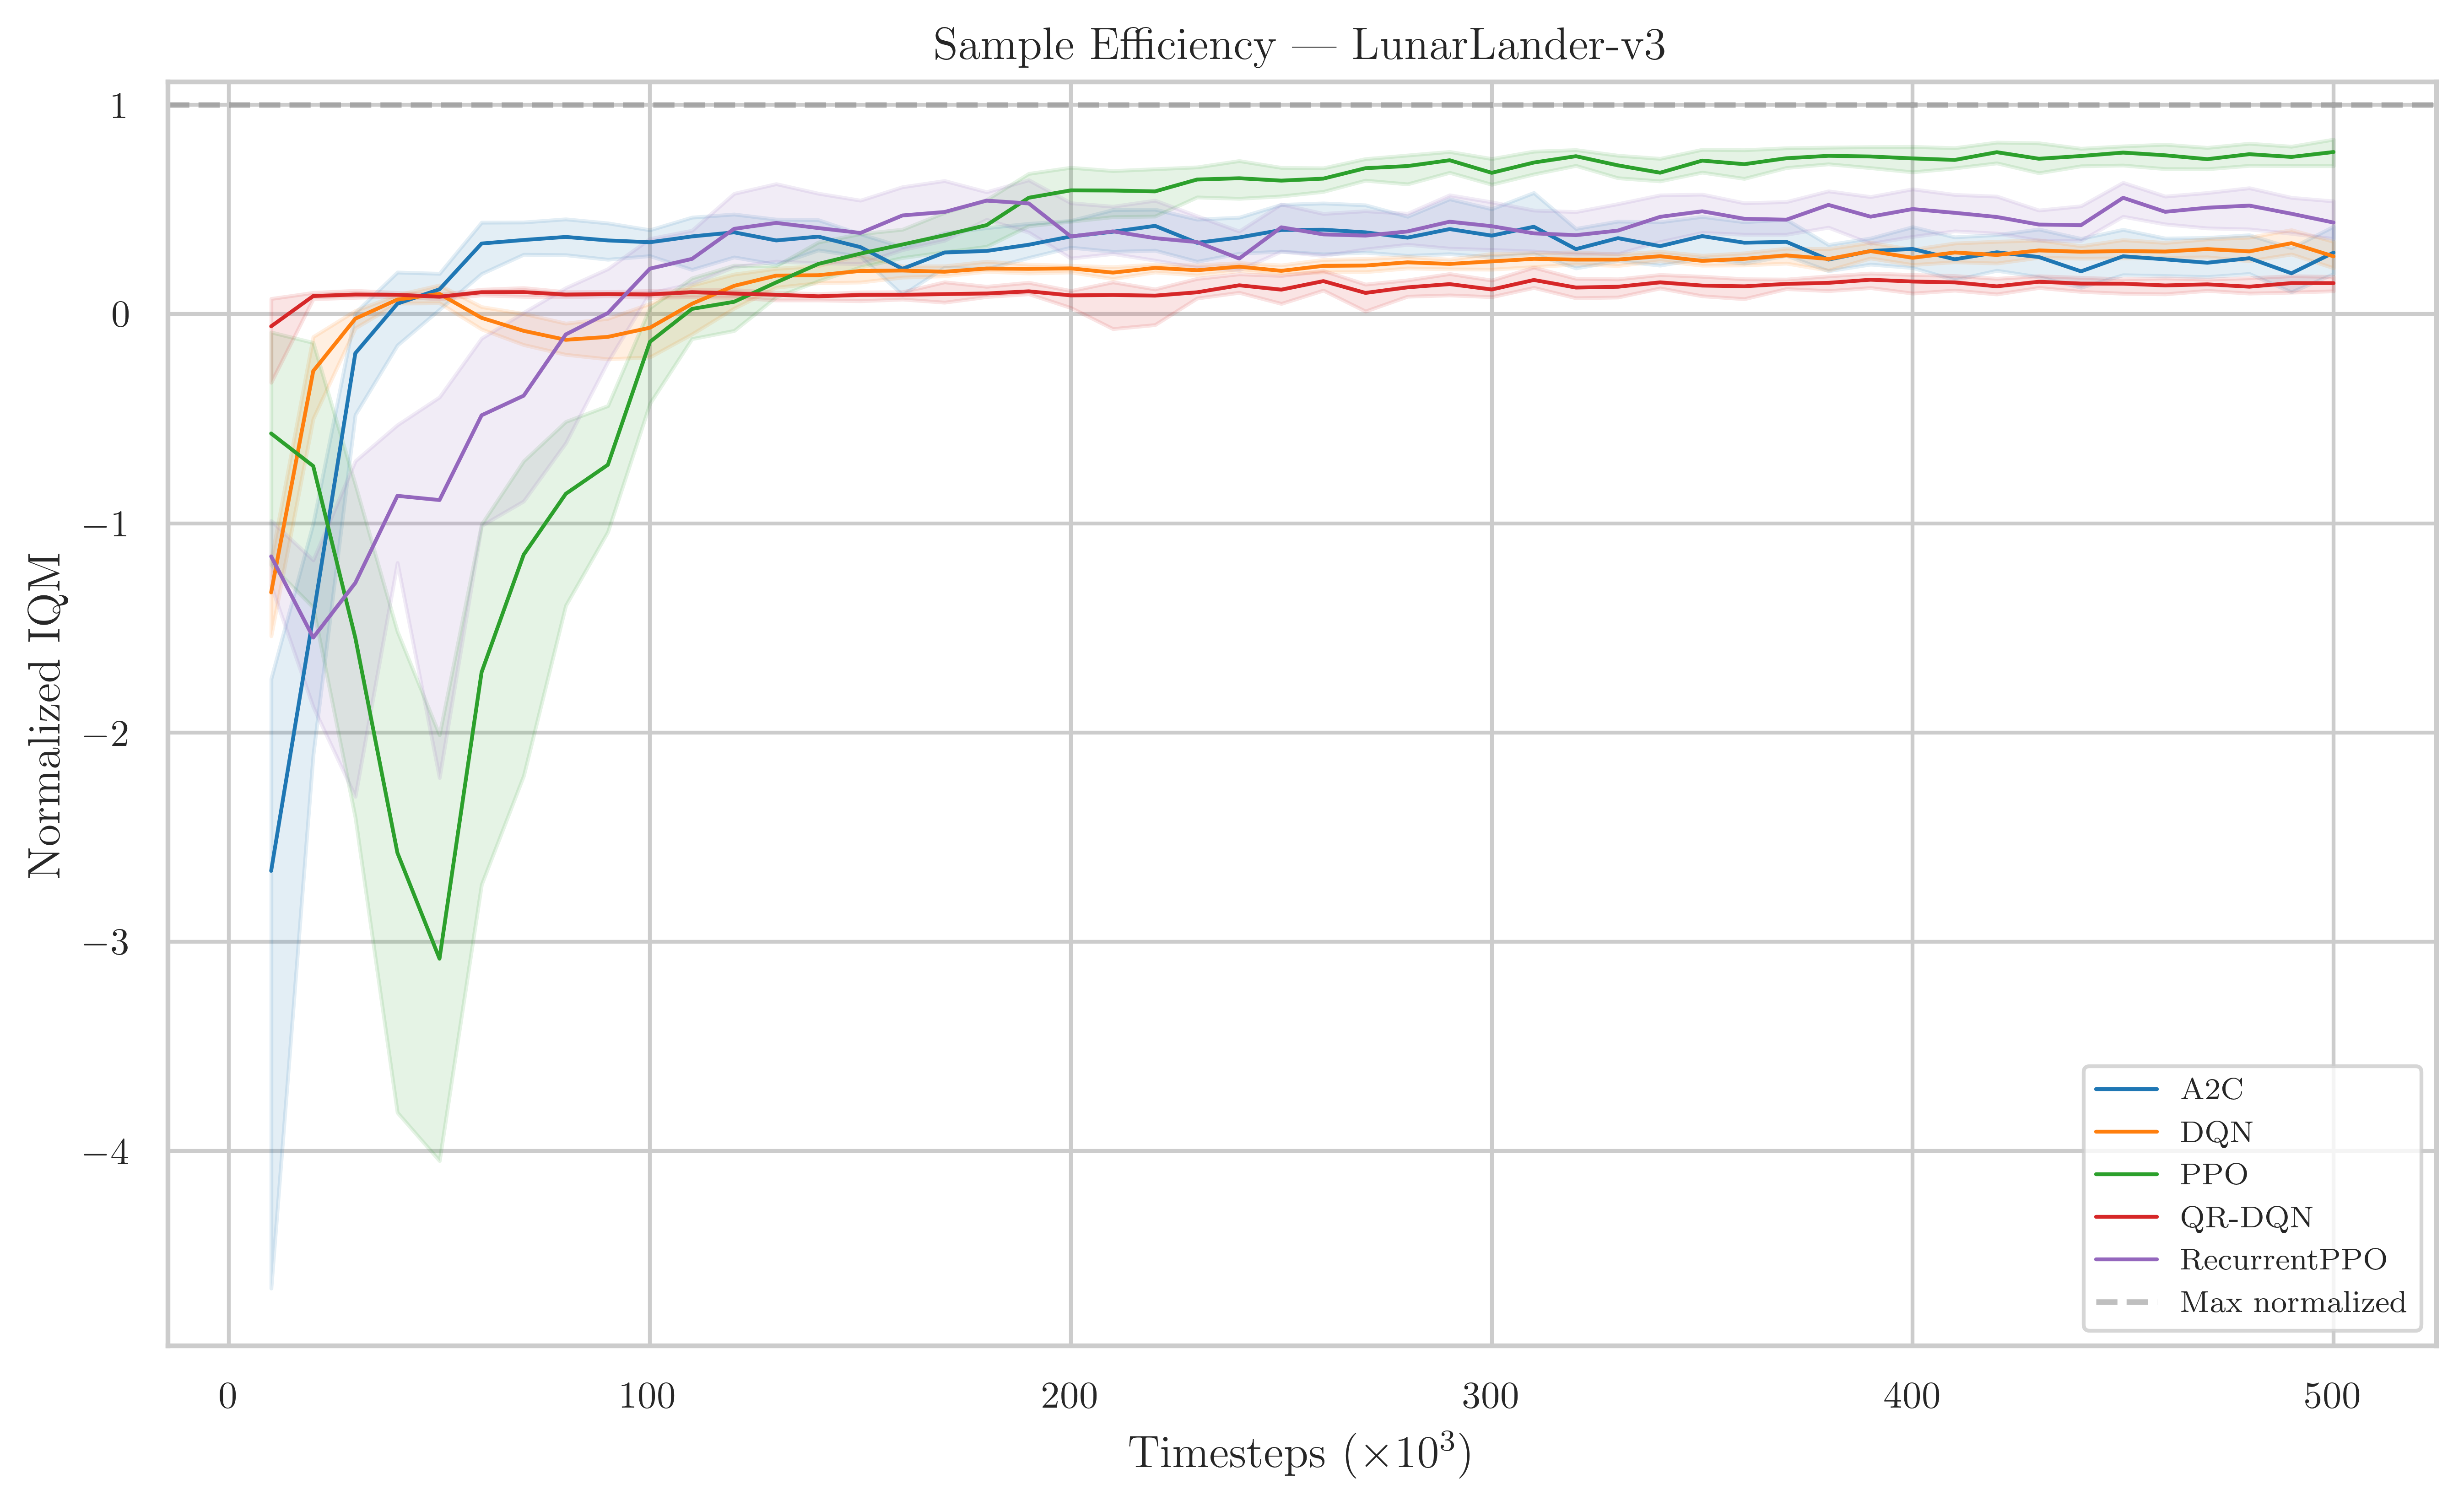
\includegraphics[width=\linewidth]{4_exp1_classic_control/assets/sample_efficiency_lunarlander-v3.png}
    \caption{LunarLander-v3}
    \label{fig:se-lunarlander}
  \end{subfigure}

  \vspace{0.5em}
  \begin{subfigure}[b]{0.5\linewidth}
    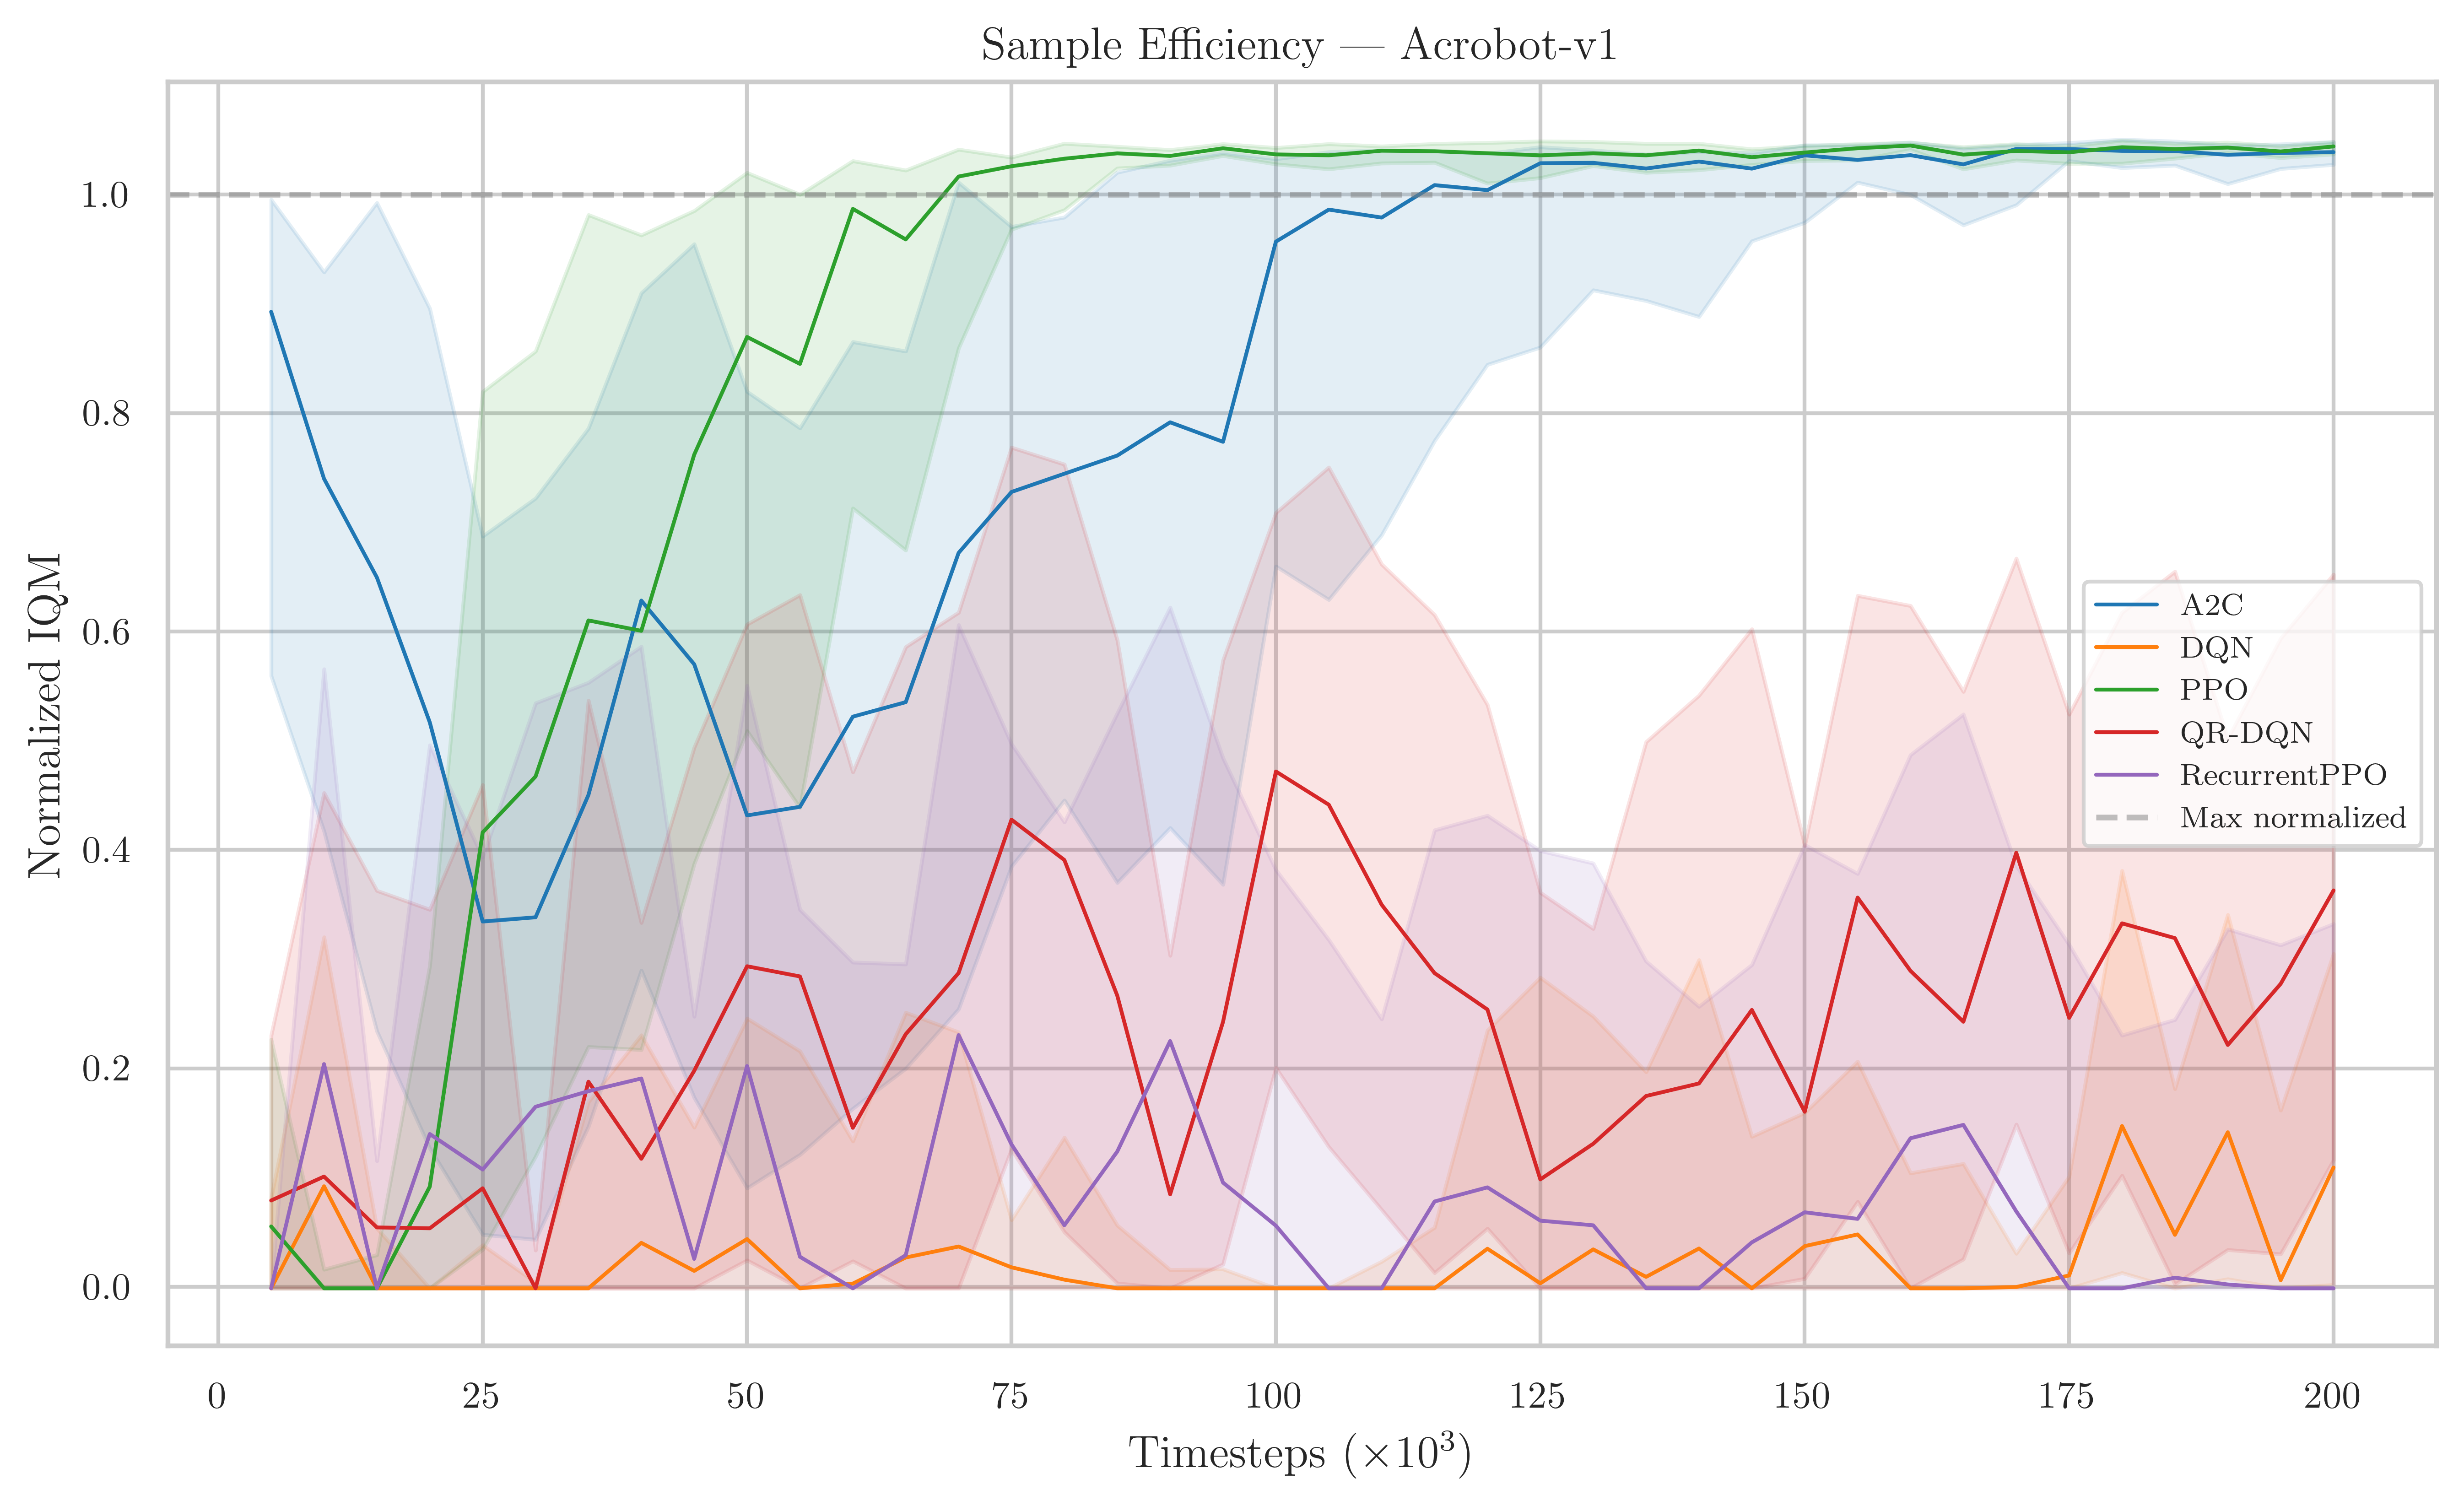
\includegraphics[width=\linewidth]{4_exp1_classic_control/assets/sample_efficiency_acrobot-v1.png}
    \caption{Acrobot-v1}
    \label{fig:se-acrobot}
  \end{subfigure}
  % \hfill
  % \begin{subfigure}[b]{0.48\linewidth}
  %   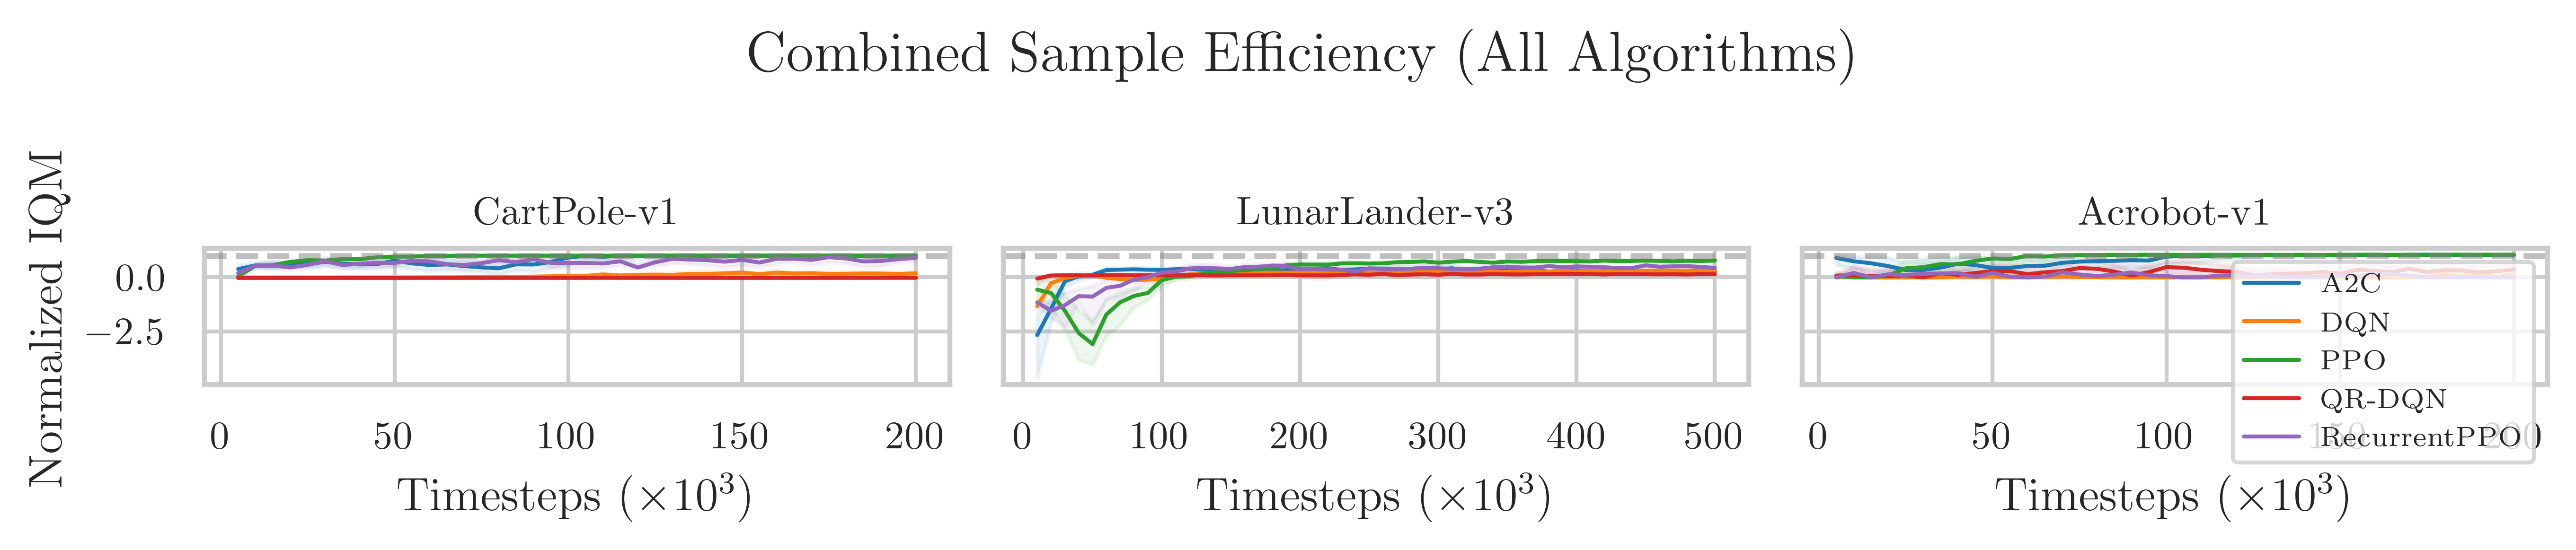
\includegraphics[width=\linewidth]{4_exp1_classic_control/assets/combined_sample_efficiency.png}
  %   \caption{Combined (normalised)}
  %   \label{fig:se-combined}
  % \end{subfigure}
  \caption[EXP1: Sample efficiency per environment]{Sample efficiency (normalised AUC) per environment.
           PPO clearly leads in all 3 environments.}
  \label{fig:sample-eff}
\end{figure}

Table~\ref{tab:sample-eff} reports the normalised AUC values. PPO achieves
the highest sample efficiency on CartPole ($0.910$) and Acrobot ($0.853$).
On LunarLander, all algorithms achieve low AUC ($0.12$--$0.24$),
reflecting the difficulty of this environment.

\begin{table}[htbp!]
\centering
\caption[EXP1: Sample efficiency AUC]{Sample efficiency (normalised AUC) per environment.}
\label{tab:sample-eff}
\begin{tabular}{lccc}
\toprule
\textbf{Algorithm} & \textbf{CartPole-v1} & \textbf{LunarLander-v3}
                   & \textbf{Acrobot-v1} \\
\midrule
PPO    & 0.910 & 0.226 & 0.853 \\
A2C    & 0.782 & 0.238 & 0.801 \\
RPPO   & 0.685 & 0.225 & 0.075 \\
DQN    & 0.075 & 0.169 & 0.022 \\
QR-DQN & $-0.025$ & 0.115 & 0.229 \\
\bottomrule
\end{tabular}
\end{table}

\subsection{Pairwise Probability of Improvement}
\label{sec:poi}

Table~\ref{tab:poi} and Figure~\ref{fig:poi} report the pairwise probability of improvement $P(A > B)$, averaged across environments. PPO has $P > 0.89$ against every other algorithm.


\begin{table}[htbp!]
\centering
\caption[EXP1: Pairwise probability of improvement]{Pairwise probability of improvement $P(\text{row} > \text{col})$,
         averaged across environments.}
\label{tab:poi}
\begin{tabular}{lccccc}
\toprule
         & \textbf{PPO} & \textbf{A2C} & \textbf{RPPO}
         & \textbf{DQN} & \textbf{QR-DQN} \\
\midrule
PPO    & ---   & 0.656 & 0.896 & 1.000 & 1.000 \\
A2C    & 0.344 & ---   & 0.642 & 0.830 & 0.939 \\
RPPO   & 0.104 & 0.358 & ---   & 0.692 & 0.744 \\
DQN    & 0.000 & 0.170 & 0.308 & ---   & 0.721 \\
QR-DQN & 0.000 & 0.061 & 0.256 & 0.279 & ---   \\
\bottomrule
\end{tabular}
\end{table}

\begin{figure}[htbp!]
  \centering
  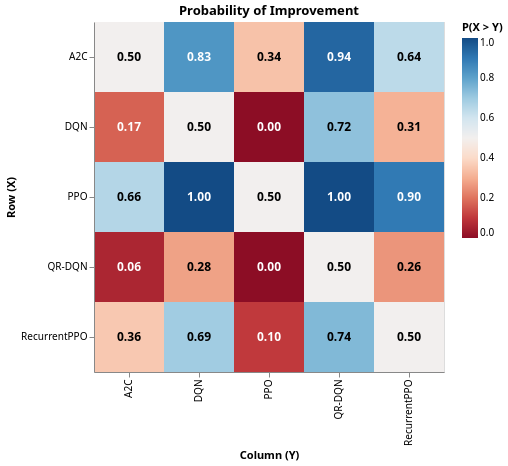
\includegraphics[width=0.8\linewidth]{4_exp1_classic_control/assets/prob_of_imporovement.png}
  \caption[EXP1: Probability of improvement heatmap]{Probability-of-improvement heatmap. PPO dominates all pairwise
           comparisons. DQN vs QR-DQN is the closest pairing ($0.72$).}
  \label{fig:poi}
\end{figure}

\subsection{Wall-Clock Timing Analysis}
\label{sec:timing}

\begin{figure}[htbp!]
  \centering
  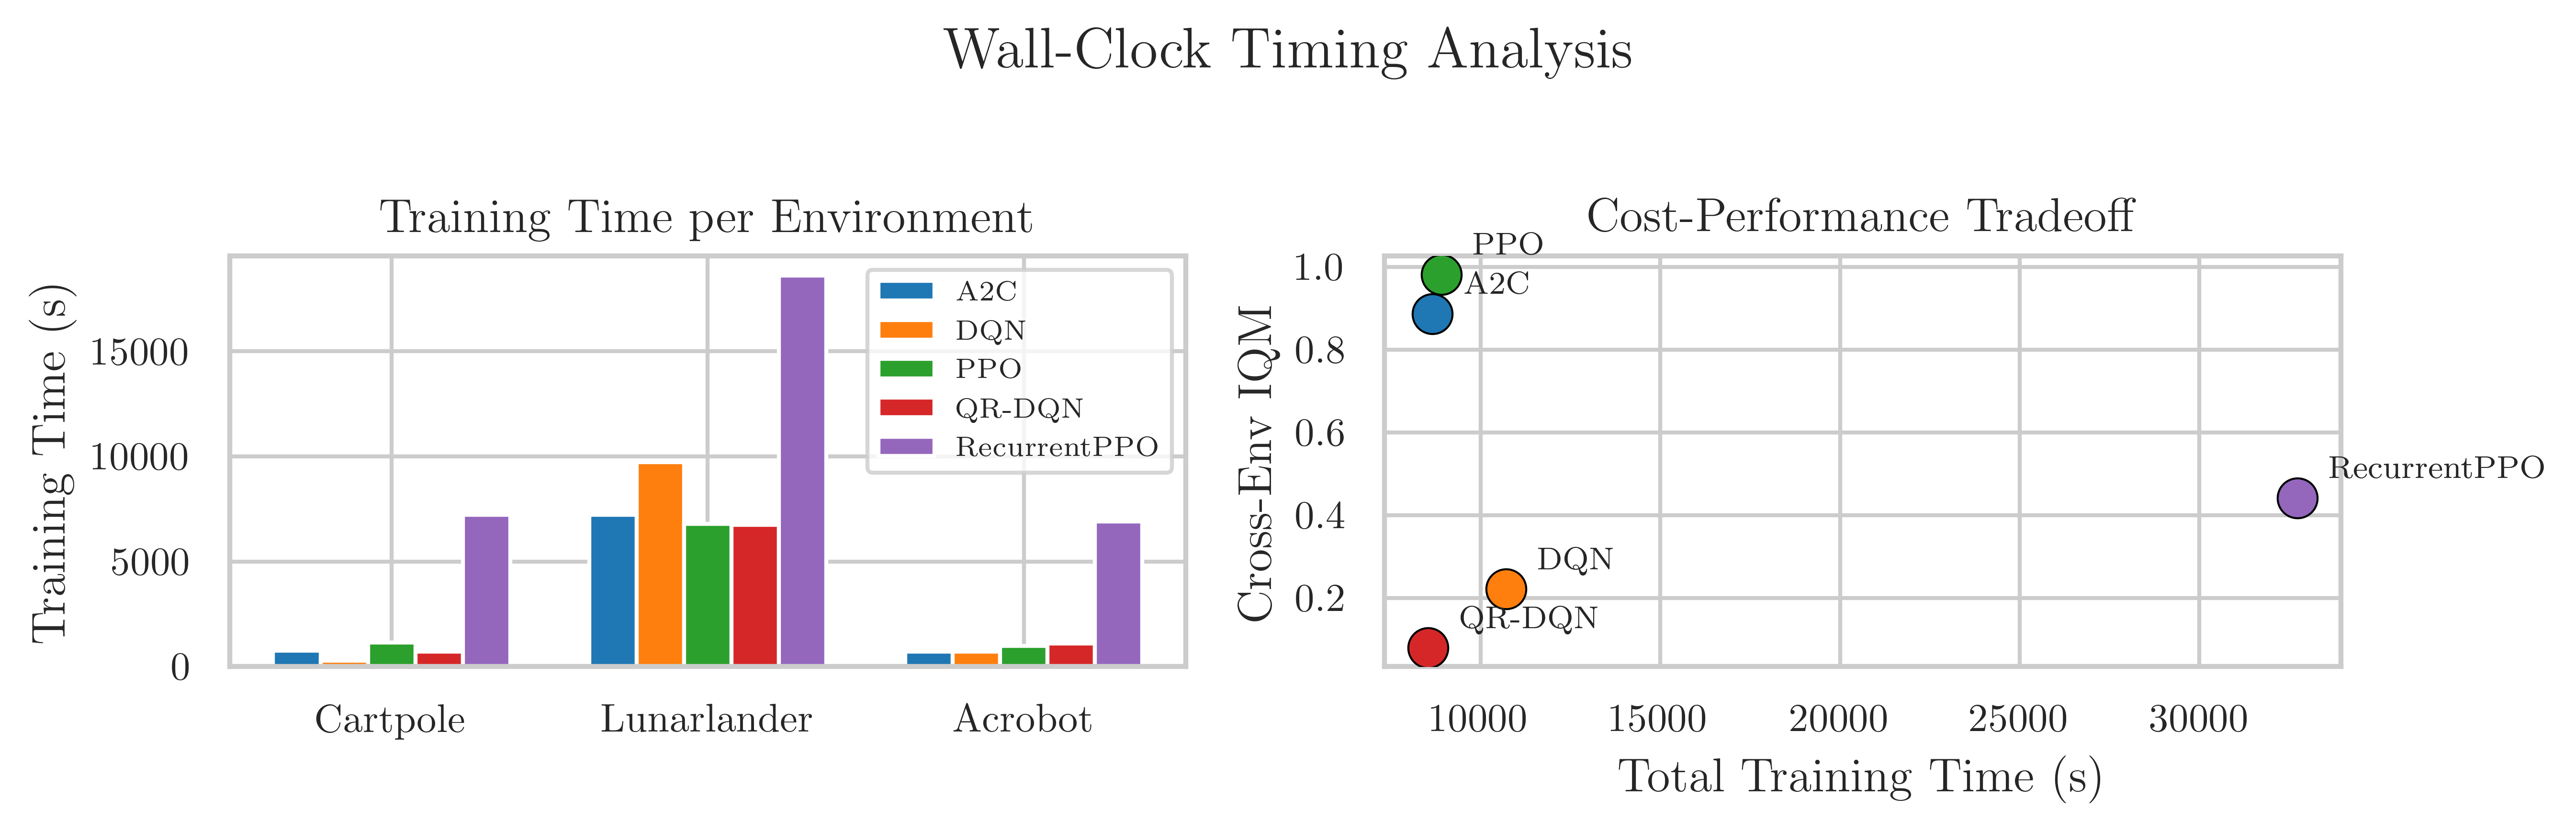
\includegraphics[width=\linewidth]{4_exp1_classic_control/assets/timing_analysis.png}
  \caption[EXP1: Wall-clock training time]{Wall-clock training time per algorithm and environment. RPPO
           is $3$--$4\times$ slower than all other algorithms due to the
           recurrent architecture.}
  \label{fig:timing}
\end{figure}

%% ------------------------------------------------------------------
\section{Key Findings: Expectations vs Reality}
\label{sec:key-findings}

Looking back at the hypotheses in Section~\ref{sec:hypotheses}, the
results contained both confirmations and genuine surprises.

\paragraph{PPO dominance was expected; the margin was not.}
I expected PPO to perform well, but I did not expect it to rank first
on \emph{every} aggregate metric (IQM $0.981$, optimality gap $0.078$)
with $P(\text{PPO} > X) \ge 0.656$ against every competitor. On CartPole
it achieves zero-variance convergence; on Acrobot it slightly exceeds
the theoretical maximum. Its only relative weakness is LunarLander, where
it still leads (IQM $0.768$) but with moderate variance. PPO's clipped
surrogate objective appears to provide a level of robustness that the
other algorithms simply cannot match under default hyperparameters.

\paragraph{A2C's LunarLander collapse.}
A2C matches PPO on two of three environments (IQM $\ge 1.0$ on CartPole
and Acrobot) and is among the cheapest to train. But its IQM of $0.303$
on LunarLander, with an IQR of $120.9$ raw-reward units, reveals a
fundamental fragility: A2C's single-step advantage estimates are too
noisy for the longer horizon, and the outcome becomes a coin flip
depending on the seed. Cross-environment IQM ($0.886$) is substantially
below PPO ($0.981$), and the pairwise probability of A2C beating PPO is
only $0.344$.

\paragraph{DQN family failure --- the biggest surprise.}
I expected DQN to solve CartPole, its own benchmark. It did not.
DQN achieves cross-environment IQM $0.222$; QR-DQN is worse at $0.080$.
This is not because DQN is a bad algorithm---it is because SB3's default
hyperparameters allocate a large fraction of the budget to replay-buffer
warm-up and $\varepsilon$-greedy exploration, leaving insufficient
learning iterations. QR-DQN's distributional head adds representational
capacity but requires more data to learn, making the budget problem
worse. The lesson is that \emph{off-policy methods on low-dimensional
tasks are sample-hungry in ways that default configurations do not
accommodate}.

\paragraph{RPPO's Acrobot catastrophe --- more capacity $\neq$ better.}
Despite sharing PPO's objective, RPPO's LSTM policy is $3.5\times$
slower to train and fails catastrophically on Acrobot (IQM $-0.001$),
where 12 of 15 seeds remain at the random-policy floor. On LunarLander,
RPPO outperforms A2C (IQM $0.444$ vs.\ $0.303$), suggesting that the
recurrence provides a small advantage on tasks with longer temporal
dependencies. But its overall ranking (IQM $0.442$, optimality gap
$0.531$) makes it a poor default choice for fully-observed MDPs.

\paragraph{Budget fairness caveat.}
A recurring theme is that the fixed training budgets (200K--500K steps)
may disadvantage off-policy algorithms that require warm-up phases.
A fairer comparison would extend the budget or include a wall-clock
normalised analysis. However, the budgets used here are typical of
the classic-control literature, and the results reflect what a
practitioner would observe when running these algorithms
``out of the box''.

{\color{red} \paragraph{Comparison with published benchmarks.}
PPO's dominance on all three environments is consistent with the reliability of on-policy methods reported in the literature \citep{schulman2017ppo}. The failure of DQN and QR-DQN at these budgets aligns with documented sensitivities of off-policy methods to training duration \citep{henderson2018matters}: without sufficient steps to warm up the replay buffer, value-based methods fail to learn regardless of their eventual capability ceiling.}

%% ------------------------------------------------------------------
{\color{red} \section{Threats to Validity}}
\label{sec:threats}

Several limitations constrain the generalisability of these results:
\begin{itemize}
  \item \textbf{Small environment suite ($M = 3$).} Cross-environment
        aggregates describe only these three tasks and should not be
        interpreted as general claims about algorithm families
        \citep{agarwal2021precipice, patterson2024edrl}.
  \item \textbf{Default hyperparameters.} No per-algorithm tuning was
        performed. DQN and QR-DQN may benefit significantly from adjusted
        learning rates, replay buffer sizes, or longer training budgets.
  \item \textbf{Fixed training budget.} The budgets (200K--500K steps)
        may be insufficient for off-policy algorithms that require a
        warm-up phase. A fairer comparison would either extend the budget
        or include a wall-clock normalised analysis.
  \item \textbf{CPU-only execution.} All experiments ran on CPU. GPU
        acceleration would reduce absolute training times but would not
        change the relative algorithmic comparison (deterministic seeding
        is CPU-only in PyTorch).
  \item \textbf{Fully-observed MDPs only.} RPPO's LSTM was never given
        an environment where memory is genuinely needed. Including a
        POMDP task would provide a fairer assessment of recurrent
        architectures.
\end{itemize}

These limitations are addressed further in Chapter~\ref{chap:evaluation}.

\section{Discussion}
\label{sec:discussion}

\paragraph{Future work.}
Extending this evaluation to continuous-action environments
(e.g., Pendulum-v1, BipedalWalker-v3) and including SAC and TD3 would
provide a more complete picture of the DQN-vs-actor-critic divide.
Additionally, a hyperparameter sensitivity analysis would clarify
whether the DQN-family's poor performance is inherent or an artefact
of the default configuration.


